\documentclass[11pt, a4paper, authoryear]{article}
%% \documentclass[coverpage]{myproposal}

\title{Distributed Programming\\ with Types and Supervision Tree: 
\\ Third Year PhD Progress Report}
\author{Jiansen HE}


\usepackage{comment}
\usepackage{natbib} 
%% \usepackage[style=alphabetic]{biblatex}
%% \usepackage[authoryear]{natbib}
%% \PassOptionsToPackage{authoryear}{natbib}
%% \usepackage{caption}
\usepackage{graphicx}
\usepackage{subfigure}
\usepackage{subcaption}
\usepackage{url}

\usepackage{paralist}
\usepackage[pdfpagelabels]{hyperref}
\usepackage[all]{hypcap}
\usepackage{verbatim}
\usepackage{array}
\usepackage{float}
\usepackage{multirow}
% \usepackage{rotating}
\usepackage{multicol}
\usepackage{longtable}
\usepackage{pdfpages}

\usepackage{listings} 	
% "define" Scala
\lstdefinelanguage{scala}{
  morekeywords={abstract,case,catch,class,def,%
    do,else,extends,false,final,finally,%
    for,if,implicit,import,match,mixin,%
    new,null,object,override,package,%
    private,protected,requires,return,sealed,%
    super,this,throw,trait,true,try,%
    type,val,var,while,with,yield},
  otherkeywords={=>,<-,<\%,<:,>:,\#,@},
  sensitive=true,
  morecomment=[l]{//},
  morecomment=[n]{/*}{*/},
  morestring=[b]",
  morestring=[b]',
  morestring=[b]"""
}


\usepackage{color}
\definecolor{dkgreen}{rgb}{0,0.6,0}
\definecolor{gray}{rgb}{0.5,0.5,0.5}
\definecolor{mauve}{rgb}{0.58,0,0.82}
 
% Default settings for code listings
\lstset{frame=tb,
  language=scala,
  aboveskip=3mm,
  belowskip=3mm,
  showstringspaces=false,
  columns=flexible,
  basicstyle={\small\ttfamily},
  numbers=left, % none,
  numbersep=2pt,
  numberstyle=\tiny\color{gray},
  keywordstyle=\color{blue},
  commentstyle=\color{dkgreen},
  stringstyle=\color{mauve},
  frame=none, % single,
  breaklines=true,
  breakatwhitespace=true,
  tabsize=2,
  captionpos=b
}



\begin{document}

%% \title{Distributed Programming with Types and OTP Design Principles: \\ Second Year Review}
%% \author{Jiansen HE}
%% \author{ \hspace{2.8 cm} Jiansen HE\newline \\  Supervised by\\ Professor Philip Wadler \\ Professor Phil Trinder \ \ \         \\ \ \ \ Professor Donald Sannella}
%% \institutes{The Laboratory for Foundations of Computer Science}
% \date{31 Aug 2013}
\maketitle
%% \tableofcontents
%% aim&objectives 	progress 		research problems & solution	evaluation	plan


\abstract{This report reviews objectives and progress of my PhD project.  
Main research problems have been solved during the process of designing and 
implementing the TAkka library.  The TAkka library has been evaluated in terms 
of correctness, expressiveness, and scalability.  To help the design of 
applications with a high reliability, the TAkka library is also shipped with 
tools for debugging and monitoring purposes.

Statistic analysis shows that it is impractical to measure the reliabilities 
of a system with low failure rate.  I propose to extend the scope of this 
research to include a formal specification of supervision tree. The 
specification gives a methodology to derive the reliability of a system built 
using supervision tree from the dependencies of nodes and the reliabilities of 
individual nodes.}



\section{Project Motivation and Objectives}

The aim of this PhD project is to {\it study how types and the 
supervision principle can be merged to help the construction of reliable 
distributed systems }.  This project intends to explore factors that encourage 
programmers to employ types and good programming principles.  To this end, the 
following iterative and incremental tasks are set.

\begin{enumerate}
  \item To identify some applications implemented in Erlang or Akka using the 
supervision principles.  Those examples will be served as references to 
evaluate frameworks that support distributed programming.  Candidate examples 
shall cover a wide range of aspects in distributed programming, including but 
not limited to 
    \begin{inparaenum} [(a)]
      \item transmitting messages and potentially computation closures, 
      \item modular composition of distributed components, 
      \item default and extensible failure recovery mechanism, and
      \item dynamic topology and hot code swapping.
    \end{inparaenum}
    
  \item To implement a library, TAkka, that supports actor programming and the 
supervision principles in a strongly typed setting.  Basic components of the 
library may be built on top of Akka\citep{akka_doc} in the case that repeated 
implementation could be avoided.  Comparing to the Akka library, the new library 
should be able to prevent more forms of type errors at earlier development 
stages.
    
  \item To re-implement identified applications using the library developed in 
task 2.  The primary purpose of this task is to be aware of the strengths and 
limitations of using strongly and weakly typed supervision libraries.  As a 
research which contains certain levels of overlaps with other existing and 
evolving frameworks, this research should distinguish itself from others by 
devised solutions to some problems which are difficult to be solved by 
alternatives.

  \item To evaluate how different supervision libraries meet the demands of 
distributed programming.  This project suggests evaluating libraries with
respects to efficiency, scalability, and reliability.
\end{enumerate}


%% Progress Overview
\section{Progress Review}

The main topic of this research was set as the result of the background study 
in the first year.  During the second year, the research objectives and the 
design of the TAkka library were refined in quarterly reviews.  By the end of 
the second year, I had
\begin{inparaenum}[\itshape a\upshape)]
\item implemented key components of the TAkka library;
\item proposed and implemented a novel typed nameserver that maps each typed 
symbol to typed a value of corresponding type;
\item demonstrated how to solve the type pollution problem using 
type-parameterized actor and subtyping; and 
\item proposed a methodology for evaluating libraries supporting the 
supervision principle.
\end{inparaenum} 

The third year is focused on the methodology for evaluating TAkka and other 
libraries that support the supervision principle.  In short,


\begin{itemize}
  \item The correctness and the expressiveness of the TAkka library is 
evaluated by porting a selection of small and medium sized applications written 
in Erlang and Akka.
  \item The scalability of sample applications written in TAkka and Akka is 
compared regarding to speed-up and throughput increases.  Benchmark examples 
for speed-up measurement are selected from the Bencherl project and tested on 
the Beowulf cluster at the Heriot-Watt University.  The example for throughput 
measurement is selected from the Techempower web framework benchmarks
\citep{techempower} and is tested using Amazon EC2 instances with a Load 
Balancer.
  \item The reliability of a TAkka application can be tested by using the 
ChaosMonkey library and the SupervisionView library.  A chaos monkey test 
assesses the robustness of a TAkka application by randomly kills actors.  The 
SupervisionView library can be used to monitor dynamical changes of a 
supervision tree.
\end{itemize}

The design, implementation, and evaluation of TAkka libraries are elaborated in 
the attached paper.



\section{Measuring Reliability}

Due to the nature of library development, we cannot assure the reliability of 
applications built using the supervision principle; nor the achieved high 
reliability of large Erlang applications can indicate that a newly implemented 
application using the supervision principle will have a desired reliability.  
To help software developers identifying bugs of their applications, 
the ChaosMonkey library and the SupervisionView library are shipped with TAkka. 
 However, a quantitative measurement of software reliability under operational 
environment is still desired in practice.  To solve this problem, two 
approaches are discussed in the attached research proposal.

The first approach is measuring the target system as black-box.  Unfortunately, 
\citep{Littlewood93} shows that even a long time failure-free observation 
itself does not suggest the software system will achieve a high reliability in 
the future.  I attempted to replace \citep{Littlewood93}'s single-run experiment 
by 
iterative experiment so that the required experiment time for some applications 
can be reduced.  Unfortunately, in most cases, predicting the reliability of a 
system with low failure rate is still impractical.  Therefore, I proposed the 
second approach which focuses on applications built using the supervision 
principle.

The second approach is giving a specification of actor-based supervision tree 
and measuring the reliability of a supervision tree as the accumulated result 
of reliabilities of its sub-trees. 
By eliminating language features not related to supervision, both the worker 
node and the supervisor node in a supervision tree can be modelled as  
Deterministic Finite Automata.  Analysis shows that various of
supervision trees can be modelled by a supervision tree that only contains 
simple worker node and simple supervisor node.  More importantly, the 
reliability of a node in the proposed model is simply defined as the possibility 
that the node is in its {\bf Free} state, in which it can react to a request.  
To accomplish this study, following problems need to be solved:
\begin{itemize}
  \item What are possible dependencies between nodes? For each dependency,
what is the algebraic relationship between the reliability of a sub-tree
and reliabilities of individual nodes?
  \item Based on the above result, how to calculate the overall reliabilities
of a supervision tree? When will the reliability be improved by using
supervising tree, and when will not?
  \item Given the reliabilities of individual workers and constraints between
them, is there an algorithm to give a supervision tree which gives a desired 
reliability?  If not, can we determine if the desired reliability is not
achievable?
\end{itemize}


\newpage

\section{Timeline for Completing Researches}


\paragraph{September 2013}

\begin{itemize}
  \item Complete the TAkka paper.  The target venue will be ECOOP. The deadline 
for ECOOP14 Research Papers has not been announced. The deadline for ECOOP13 
Research Papers is 22 Dec 2012.
  \item Write a technical memo about the proposed specification of 
supervision tree.  The specification will focus on actor-based systems.  
Candidate Erlang and Akka examples will be identified to check the coverage of 
the specification.
\end{itemize}

\paragraph{December 2013}
\begin{itemize}
  \item Document the design, implementation, and evaluation of the TAkka 
library in thesis format.
  \item Complete the specification for supervision tree.  The specification 
will includes a comprehensive study on the relationship between system 
reliability and common dependencies between actors.
  \item Write a brief proposal on extending the scope of the specification for 
supervision tree so that it can model a wider range of systems.  The proposal 
will include the target scope of the generalisation, any modifications to the 
specification for actor-based system, and examples for the evaluation process.
  \item Write up a quarterly review report about the above tasks.  The purpose 
of the quarterly review is tracking the direction and progress of my PhD 
research project.  The review report will discuss whether extending the scope 
of the specification for supervision tree should be part of the PhD research.
\end{itemize}


\paragraph{March 2014}
\begin{itemize}
  \item Document the specification for supervision tree in thesis format. 
\end{itemize}

\paragraph{June 2014}
\begin{itemize}
  \item Complete the thesis writing.
\end{itemize}

\bibliographystyle{abbrvnat}
\bibliography{Aug2013}

\appendix
%% This is LLNCS.DEM the demonstration file of
% the LaTeX macro package from Springer-Verlag
% for Lecture Notes in Computer Science,
% version 2.4 for LaTeX2e as of 16. April 2010
%
\documentclass[authoryear,preprint]{sigplanconf}


%
\usepackage{makeidx}  % allows for indexgeneration
\usepackage{comment}



%% \usepackage[style=alphabetic]{biblatex}
% \usepackage[authoryear,sectionbib]{natbib}
%% \PassOptionsToPackage{authoryear}{natbib}
%% \usepackage{caption}
\usepackage{graphicx}
\usepackage{subfigure}
\usepackage{url}

\usepackage{paralist}
\usepackage{verbatim}
\usepackage{array}
\usepackage{float}
\usepackage{multirow}
% \usepackage{rotating}
\usepackage{multicol}
\usepackage{longtable}

\usepackage{listings} 	
% "define" Scala
\lstdefinelanguage{scala}{
  morekeywords={abstract,case,catch,class,def,%
    do,else,extends,false,final,finally,%
    for,if,implicit,import,match,mixin,%
    new,null,object,override,package,%
    private,protected,requires,return,sealed,%
    super,this,throw,trait,true,try,%
    type,val,var,while,with,yield},
  otherkeywords={=>,<-,<\%,<:,>:,\#,@, <:<},
  sensitive=true,
  morecomment=[l]{//},
  morecomment=[n]{/*}{*/},
  morestring=[b]",
  morestring=[b]',
  morestring=[b]"""
}


\usepackage{pxfonts}
\usepackage{color}
\definecolor{dkgreen}{rgb}{0,0.6,0}
\definecolor{gray}{rgb}{0.5,0.5,0.5}
\definecolor{mauve}{rgb}{0.58,0,0.82}
 
% Default settings for code listings
\lstset{frame=tb,
  language=scala,
  aboveskip=3mm,
  belowskip=3mm,
  showstringspaces=false,
  columns=flexible,
  basicstyle={\small\ttfamily},
  numbers=left, % none,
  numbersep=2pt,
  numberstyle=\tiny\color{gray},
  keywordstyle=\bfseries\color{black},
  commentstyle=\color{dkgreen},
  stringstyle=\color{black},
  frame=none, % single,
  breaklines=true,
  breakatwhitespace=true,
  tabsize=2,
  captionpos=b
}

\usepackage[pdfpagelabels]{hyperref}
\usepackage[all]{hypcap}


% A comment in a draft (shouldn't appear in the final version).
\newcommand{\mycomment}[1]{\(\spadesuit\){\bf #1 }\(\spadesuit\)}
% Comment this out in the draft
% \newcommand{\mycomment}[1]{}
\newcommand{\pmcomment}[1]{\comment{PM}{#1}}
\newcommand{\pwtcomment}[1]{\comment{PT}{#1}}
\newcommand{\rscomment}[1]{\comment{RS}{#1}}

% line break in table.  e.g.
% Foo bar & \specialcell{Foo\\bar} & Foo bar \\    % vertically centered
% Foo bar & \specialcell[t]{Foo\\bar} & Foo bar \\ % aligned with top rule
\newcommand{\specialcell}[2][c]{%
  \begin{tabular}[#1]{@{}c@{}}#2\end{tabular}}
  
  
\renewcommand\bibname{References}


\begin{document}

\special{papersize=8.5in,11in}
\setlength{\pdfpageheight}{\paperheight}
\setlength{\pdfpagewidth}{\paperwidth}

\conferenceinfo{CONF 'yy}{Month d--d, 20yy, City, ST, Country} 
\copyrightyear{20yy} 
\copyrightdata{978-1-nnnn-nnnn-n/yy/mm} 
\doi{nnnnnnn.nnnnnnn}
           
\titlebanner{banner above paper title}        % These are ignored unless
\preprintfooter{short description of paper}   % 'preprint' option specified.

\title{Typecasting Actors: from Akka to TAkka
}
% \subtitle{Subtitle Text, if any}

\authorinfo{Jiansen HE}
           {University of Edinburgh}
           {jiansen.he@ed.ac.uk}
\authorinfo{Philip Wadler}
           {University of Edinburgh}
           {wadler@inf.ed.ac.uk}
\authorinfo{Philip Trinder}
           {University of Glasgow}
           {Phil.Trinder@glasgow.ac.uk}

\maketitle



\begin{comment} 

Scala supports actors and message passing with the Akka library. Though Scala is 
statically typed, messages in Akka are dynamically typed (that is, of type Any). 
The Akka designers argue that using static types is "impossible" because "actor 
behaviour is dynamic", and, indeed, it is not clear that important actor 
support, such as supervision or name servers, could be implemented if messages 
are statically typed. Here we present Takka, a variant of Akka where messages 
are statically typed, and show that it is possible to implement supervisors and 
name servers in such a framework. We show it is possible to upgrade from Akka to 
Takka gradually, porting one module at a time; and we show that Takka can 
support behavioral upgrade where the new message type of an actor is a supertype 
of the old type. We demonstrate the expressiveness of Takka by rewriting a score 
of Akka applications; the percentage of lines that needs to be changed varies 
from 44\% (in a 25 line program) to 0.05\% (in a 27,000 line program), with a 
geometric mean of 8.5\%. We measure the execution speed, scalability, and 
throughput of Takka programs and show that it is comparable to Akka. [perhaps 
give precise details]

\end{comment}




\begin{abstract} 

  Scala supports actors and message passing with the Akka
  library. Though Scala is statically typed, messages in Akka are
  dynamically typed (that is, of type {\tt Any}).  The Akka designers
  argue that using static types is ``impossible'' because ``actor
  behaviour is dynamic'', and, indeed, it is not clear that important
  actor support, such as supervision or name servers, can be
  implemented if messages are statically typed. Here we present TAkka,
  a variant of Akka where messages are statically typed, and show that
  it is possible to implement supervisors and name servers in such a
  framework. We show it is possible to upgrade from Akka to TAkka
  gradually, porting one module at a time; and we show that TAkka can
  support behavioural upgrade where the new message type of an actor is
  a supertype of the old type. We demonstrate the expressiveness of
  TAkka by rewriting a score of Akka applications; the percentage of
  lines that need to be changed varies from 44\% (in a 25-line
  program) to 0.05\% (in a 27,000-line program), with a geometric mean
  of 8.5\%. We measure the execution speed, scalability, and
  throughput of TAkka programs and show that they are comparable to Akka.

\end{abstract}

% \vspace{-5pt}
\section{Introduction}

Can the benefits of static typing extend to message passing?

A distinguishing feature of Scala is its sophisticated static type
system.  A distinguishing feature of modern computing is its reliance
on communication.  Scala supports communication with the Akka library
\citep{akka_doc}, partly inspired by Erlang \citep{ArmstrongErlang}, which in
turn is inspired by actors and message passing \citep{Hewitt:1973}.
However, these two features do not play well together---messages
in Akka are dynamically typed (that is, of type {\tt Any}).

There are sound reasons for this design.  The Akka designers argue
that using static types is ``impossible'' because ``actor behaviour is
dynamic'' \citep{Kuhn11, Kuhn12}.  The design of Akka is
inspired by the Erlang OTP Design Principles, including supervision
trees to ensure reliability, and Erlang is dynamically typed.  Since
supervision is generic---a supervision framework is instantiated to
processes transmitting many types of messages---it is not immediately
clear whether static typing is sensible.  All supervised actors need
to accept a fixed set of system messages, such as Poison Pill (to kill a
superised actor), and it is not clear how to incorporate these into
statically typed messages.  An important part of distributed
infrastructure is a name server, which maps names to actors, and
while it is easy to build a map from names to entities of
dynamic type, it is again not clear how to build a map to entities
with different static types.

This paper introduces TAkka, a variant of Akka with statically typed
messages.  It turns out that each of the issues above can be resolved
straightforwardly.  Each actor is parameterised on the type of
messages it handles.  In addition, each actor can also receive system
messages, such as Poison Pill, which are handled by the supervision
framework.  The name server uses Scala ``manifest'' types to support a
name server that maps names to actors with different static types.

It is essential that a large program can be upgraded incrementally,
one module at a time, rather than requiring a monolithic change to 
all modules simultaneously---a principle we summarise by the motto
``Evolution, not Revolution''.  TAkka is designed to support
incremental change, and, in particular, a service written in Akka
can interact with a client written in TAkka, and vice versa.
Backward compatibility is supported, because TAkka actors inherit
from Akka actors.

In a system with multiple components, different components may require
different interfaces; since all messages are received in the same
mailbox, a naive approach would be to set the type to the union of all
the interfaces, causing each component to see a type containing
messages not intended for it---an issue we dub the Type Pollution
Problem.  Fortunately, the problem may be avoided by exploiting
subtyping to publish a different interface to each layer.

To evaluate the expressiveness of our system, we rewrite a score of
Akka applications in TAkka.  The percentage of lines that need to be
changed varies from 44\% (in a 25-line program) to 0.05\% (in a
27,000-line program), with a geometric mean of 8.5\%.

We confirm that Akka and TAkka have comparable performance in terms of
throughput, runtime, and scalability.  We compare the throughput of
Play and Socko implementations written in both systems, and show the
throughput of Akka and TAkka is on average within 8.75\% of each
other.  We compare the runtime and scalability of six BenchErl
benchmarks, and show that the runtimes of Akka and TAkka are on
average within 8.89\% of each other, and that they have similar
scalability profiles.

The paper makes the following contributions.

\vspace{-8pt}
\begin{itemize}\setlength{\itemsep}{0pt}
\item We contrast Akka and TAkka, illustrating the differences with a
  simple application, a supervised calculator (Section~\ref{actor}).

\item We review the Akka API, and present the corresponding TAkka API
  (Section~\ref{takka_design}).

\item We describe the construction of a name server that maps names to
  actors of different static types (Section~\ref{nameserver}).

\item We demonstrate that TAkka supports the principle of
  ``Evolution, not Revolution'', by showing how Akka and TAkka code
  for the supervised calculator can interact (Section~\ref{evolution}).

\item We illustrate the Type Pollution Problem and its solution
  on an instance of the Model-View-Controller pattern (Section~\ref{type_pollution}).

\item We rewrite a score of Akka programs in TAkka, and measure the
  differences in line count (Section~\ref{expressiveness}).

\item We compare the throughput of Play and Socko implementations
  written in both Akka and TAkka, and we compare the runtime and
  performance of a half-dozen BenchErl benchmarks written in both
  Akka and TAkka (Section~\ref{efficiency}).
\end{itemize}
\vspace{-5pt}
Section~\ref{conclusion} concludes.


\section{Actors and Their Supervision}
\label{actor}

The Akka library \citep{akka_doc} implements actor programming and
makes supervision obligatory. As an introduction to Akka,
Figure~\ref{akka:supervisedcalculator} defines a calculator.
Each {\tt Actor} defines a {\tt receive} method that reacts to
incoming messages. Each {\tt ActorRef} references an actor, and
may be sent messages with the {\tt !} operator. Our example
program defines {\tt Multiplication} and {\tt Division} messages
(lines~5--6), a {\tt Calculator} actor which receives them
(lines~8--15), and instantiates a {\tt SafeCalculator} actor
reference which is sent such messages (lines~29--35).
(The relation between {\tt Calculator} and {\tt SafeCalculator}
is explained below.)

Akka makes supervision obligatory by restricting the manner of actor
creation.  Calling the {\tt actorOf} method of an actor context
creates a child actor supervised by that actor, forming a tree
structure (lines~23--24).  There is a system-provided guardian actor which
serves as the root of the supervision tree (lines~29--31).  (Strictly
speaking, {\tt actorOf} is invoked on an {\tt ActorContext} or {\tt
  ActorSystem}, and it is supplied with an instance of the {\tt Props}
class to specify properties of the actor to be created; details are
given in Section~\ref{actor_context}.)  Obligatory supervision unifies
the structure of actor deployment and simplifies the work of system
maintenance.

% Actors can only be initialized by passing an instance of
% {\tt Props} class to the {\tt actorOf} method, provided by {\tt
%   ActorSystem} or {\tt ActorContext}.  

The simple calculator does not consider the problematic case of dividing by~0,
where an {\tt ArithmeticException} will be raised.  We define 
a {\tt SafeCalculator} as the supervisor of {\tt Calculator}.
The {\tt receive} method of the safe calculator delegates any
messages received to the calculator (line~25), and defines a
supervisor strategy that restarts the calculator when an
{\tt ArithmeticException} is raised (lines~17--22).
% The 
% supervisor strategy of the safe calculator also specifies that its child may 
% not fail more than twice within a minute.  If the child fails more 
% frequently, the safe calculator itself will stop, and the failure will be 
% reported to its supervisor, the system guardian actor in this example.  The 
% terminal output shows that the simple calculator is restarted before messages 
% sent at line 48 and 50 are processed.  The last message sent at line 52 is 
% not processed because both calculators have been terminated due to the fact 
% that the simple calculator fails more frequently than allowed.
% The terminal output shows that the exception raised by the simple calculator is 
% handled by its supervisor and it can process new messages.


% An undefined message (line~40) is treated 
% differently in different Akka versions.  In versions 
% prior to 2.0, an Akka actor raises an exception when it processes an undefined 
% message. In recent Akka versions, an undefined message is discarded by the 
% actor and an {\tt UnhandledMessage} event is pushed to the event stream of the 
% actor system. The event stream may be subscribed to by other actors who are 
% interested in particular event messages. Our example program defines a
% handler (lines~45---50) and subscribes to the {\tt UnhandledMessage} events
% (lines~33--35).
In Akka 2.0 and later versions, an undefined message (line~40) is discarded and 
an {\tt UnhandledMessage} event is pushed to the event stream of the 
actor system. The event stream may be subscribed to by other actors who are 
interested in particular event messages. Our example program defines a
handler (lines~44---49) and subscribes to the {\tt UnhandledMessage} events
(lines~33--35).

Figure~\ref{takka:supervisedcalculator} gives an equivalent TAkka 
implementation. Code that appears in the Akka version but not the TAkka
version, or vice versa, is coloured \textcolor{blue}{blue}.  The 
TAkka {\tt Actor} class takes a type parameter, 
{\tt M}, which indicates the type of expected messages.  Correspondingly, its 
message handler, {\tt typedReceive}, has type
{\tt M => Unit}.
% Similarly, a type parameter is added to the {\tt ActorRef} class (Section~\ref{actor_ref})
% and the {\tt ActorContext} class (Section~\ref{actor_context}).
Similarly, a type parameter is added to the {\tt Props} 
class and the {\tt ActorRef} class.  An actor created from an instance of 
{\tt Props[M]} has {\tt Actor[M]}, whose corresponding actor reference 
has type {\tt ActorRef[M]}.  Messages sent to an actor reference of type {\tt 
ActorRef[M]} must have type {\tt M}.

Hence, developers only need to consider messages of the expected
type. An attempt to send a message of a type not expected by the
receiver is rejected at compile-time (line~36).  TAkka uses a typed
name server, as explained in Section~\ref{nameserver}.  When looking
up an actor by name, the expected type is provided, and if it does not
match the type of the stored actor reference then an error is raised
at run-time (lines~46---47).  In the TAkka version, there is no need to
define a handler for unexpected messages.

% \vspace{-5pt}
\section{Library Design}
\label{takka_design}

This section elaborates the design of the TAkka library, which provides type 
parameters for the Actor related classes found in Akka.  Figure~\ref{akka_api}
gives the Akka API, and Figure~\ref{takka_api} gives it TAkka counterpart.

% \vspace{-5pt}
\subsection{Actor}

A TAkka actor has type {\tt Actor[M]}.  Unlike other actor 
libraries, every TAkka actor class takes a type parameter {\tt M} which 
specifies the type of messages it expects to receive.  The same type parameter 
is used as the input type of the receive function, the type parameter of the 
actor context and the type parameter of the actor reference pointing to itself. 
TAkka uses Scala {\tt Manifest} to record type information required at runtime.

The TAkka {\tt Actor} class inherits 
the Akka {\tt Actor} trait to minimize implementation effort.  Users of the 
TAkka library, however, do not need to use any Akka Actor API.  Instead, we 
encourage programmers to use the typed interface given in Figure~\ref{takka_api}.  
The limitation of using inheritance to implement TAkka actors 
is that Akka features are still available to library users.  Unfortunately, 
this limitation cannot be overcome by using delegation because, as we have seen 
in the {\tt SupervisedCalculator} example, a child actor is created by calling the {\tt actorOf} method from 
its supervisor's actor context, which is a private field of the supervisor.  
{\tt Actor} is the only TAkka class that is implemented using inheritance. 
Other TAkka classes are either implemented by delegating tasks to Akka 
counterparts or rewritten in TAkka.  Re-implementing the TAkka 
Actor library requires a similar amount of work as implementing the Akka Actor 
library.


\begin{figure}[p]

  \begin{lstlisting}[language=scala,   escapechar=?]
package sample.?\textcolor{blue}{akka}?.SafeCalculator
import ?\textcolor{blue}{akka}?.actor.{ActorRef, ActorSystem, Props, Actor}
?\textcolor{blue}{import akka.actor.UnhandledMessage}?

case class Multiplication(m:Int, n:Int)
case class Division(m:Int, n:Int)

class Calculator extends Actor {
  def ?\textcolor{blue}{receive}? = {
    case Multiplication(m:Int, n:Int) =>
      println(m +" * "+ n +" = "+ (m*n))
    case Division(m:Int, n:Int) =>
      println(m +" / "+ n +" = "+ (m/n))
  }
}
class SafeCalculator extends Actor {
  override val supervisorStrategy =
    OneForOneStrategy() {
      case _: ArithmeticException  =>
        println("ArithmeticException Raised to: "+?\textcolor{blue}{self}?)
        Restart
    }
  val child:ActorRef = ?\textcolor{blue}{context}?.actorOf(
  				Props[Calculator], "child")
  def ?\textcolor{blue}{receive}? = {    case m => child ! m  }
}
object SafeCalculatorTest extends App {
  val system = ActorSystem("MySystem")
  val calculator:ActorRef = 
      system.actorOf(Props[SafeCalculator],
                        "calculator")

  calculator ! Multiplication(3, 1)
  calculator ! Division(10, 0)
  calculator ! Division(10, 5)
  
  ?\textcolor{blue}{  val handler = system.actorOf(Props[MessageHandler])}?
  ?\textcolor{blue}{ system.eventStream.subscribe(handler, }?
                     ?\textcolor{blue}{ classOf[UnhandledMessage]);  }?
  ?\textcolor{blue}{ calculator ! "Hello" }?
}


?\textcolor{blue}{class MessageHandler extends Actor\{}?
  ?\textcolor{blue}{def receive = \{}?
    ?\textcolor{blue}{case UnhandledMessage(message, sender, recipient) =>}?
      ?\textcolor{blue}{println("unhandled message: "+message);}?
  ?\textcolor{blue}{\}}?
?\textcolor{blue}{\}}?

/* Terminal Output:
3 * 1 = 3
java.lang.ArithmeticException: / by zero
ArithmeticException Raised to: Actor[akka://MySystem/user/calculator]
10 / 5 = 2
unhandled message: Hello
*/


    \end{lstlisting}
  \caption{Akka Example: Supervised Calculator}
  \vspace*{2 in}
  \label{akka:supervisedcalculator}
\end{figure}


\begin{figure}[p]
    \begin{lstlisting}[language=scala, escapechar=?]
package sample.?\textcolor{blue}{takka}?.SafeCalculator
import ?\textcolor{blue}{takka}?.actor.{ActorRef, ActorSystem, Props, Actor}

?\textcolor{blue}{sealed trait Operation}?
case class Multiplication(m:Int, n:Int) ?\textcolor{blue}{extends Operation}?
case class Division(m:Int, n:Int) ?\textcolor{blue}{extends Operation}?

class Calculator extends Actor?\textcolor{blue}{[Operation]}?{
  def ?\textcolor{blue}{typedReceive}? = {
    case Multiplication(m:Int, n:Int) =>
      println(m +" * "+ n +" = "+ (m*n))    
    case Division(m, n) =>
      println(m +" / "+ n +" = "+ (m/n))
  }
}
class SafeCalculator extends Actor?\textcolor{blue}{[Operation]}? {
  override val supervisorStrategy =
    OneForOneStrategy() {
      case _: ArithmeticException  =>
      println("ArithmeticException Raised to: "+?\textcolor{blue}{typedSelf}?)
      Restart
    }
  val child:ActorRef[Operation] = ?\textcolor{blue}{typedContext}?.actorOf(
  		Props[?\textcolor{blue}{Operation}?, Calculator], "child")
  def ?\textcolor{blue}{typedReceive}? = {    case m => child ! m  }
}
object SafeCalculatorTest extends App{
  val system = ActorSystem("MySystem")
  val calculator:ActorRef?\textcolor{blue}{[Operation]}? = 
        system.actorOf(Props[?\textcolor{blue}{Operation}?, SafeCalculator], 
                          "calculator")
                          
  calculator ! Multiplication(3, 1)
  calculator ! Division(10, 0)
  calculator ! Division(10, 5)                          
  //  calculator ! "Hello" 
  //    compile error:  type mismatch; found : 
  //                      String("Hello") required: 
  //    sample.takka.SupervisedCalculator.Operation
  
  ?\textcolor{blue}{System.out.println("Name server test") }?
  ?\textcolor{blue}{val calMul = system.actorFor[Multiplication]}?
                             ?\textcolor{blue}{("akka://MySystem/user/calculator")}?
  ?\textcolor{blue}{calMul ! Multiplication(3, 2)}?
  ?\textcolor{blue}{Thread.sleep(1000)}?
  ?\textcolor{blue}{val calStr = system.actorFor[String]}?
                              ?\textcolor{blue}{("akka://MySystem/user/calculator")}?
  // Exception raised before this line is reached                              
  ?\textcolor{blue}{calStr ! "Hello" }?
}
/* Terminal Output:
3 * 1 = 3
java.lang.ArithmeticException: / by zero
ArithmeticException Raised to: Actor[akka://MySystem/user/calculator]
10 / 5 = 2
Name server test
3 * 2 = 6
Exception in thread "main" java.lang.Exception: ActorRef[akka://MySystem/user/calculator] does not exist or does not have type ActorRef[String]
*/
    \end{lstlisting}
    \caption{TAkka Example: Supervised Calculator}
  \vspace*{1 in}    
    \label{takka:supervisedcalculator}
\end{figure}








\begin{figure}[!h]
\label{akka_api}
\begin{lstlisting}[language=scala, escapechar=?]
package ?\textcolor{blue}{akka}?.actor   
\end{lstlisting}
\begin{lstlisting}[language=scala, escapechar=?]
abstract class ActorRef
  def !(message: ?\textcolor{blue}{Any}?):Unit
\end{lstlisting}
\vspace{20pt}
    \begin{lstlisting}[language=scala, escapechar=?]
?\textcolor{blue}{trait }? Actor
  def ?\textcolor{blue}{receive:PartialFunction[Any, Unit]}?
  val ?\textcolor{blue}{self: ActorRef}?
  private val ?\textcolor{blue}{contrext: ActorContext}?
  var supervisorStrategy: SupervisorStrategy
\end{lstlisting}

      \begin{lstlisting}[language=scala, escapechar=?]
?\textcolor{blue}{trait}? ActorContext
   def actorOf(props: Props): ActorRef
   
   def actorOf(props: Props, name: String): ActorRef

  def actorFor(path: String): ActorRef
  
  def setReceiveTimeout(timeout: Duration): Unit
  def become(behavior: ?\textcolor{blue}{PartialFunction[Any, Unit]}?, 
  						?\textcolor{blue}{discardOld: 
Boolean = true): Unit}?
						
  ?\textcolor{blue}{def unbecome(): Unit}?

    \end{lstlisting}

    \begin{lstlisting}[language=scala, escapechar=?]
?\textcolor{blue}{final case class Props(deploy: Deploy,}?
		?\textcolor{blue}{clazz: Class[\_], }?
		?\textcolor{blue}{args: immutable.Seq[Any]) }?
    \end{lstlisting}
    \begin{lstlisting}[language=scala, escapechar=?]
object Props extends Serializable
  def apply(creator: =>Actor): Props
  def apply(actorClass: Class[_ <: Actor]): Props  
  def apply[T <: Actor]()
  		(implicit arg0: Manifest[T]): Props  
    \end{lstlisting}

    \begin{lstlisting}    
abstract class SupervisorStrategy
case class OneForOneStrategy(restart:Int = -1, 
              time:Duration = Duration.Inf)
              (decider: Throwable =>  Directive) 
              extends SupervisorStrategy
case class OneForAllStrategy(restart:Int = -1, 
              time:Duration = Duration.Inf)
              (decider: Throwable =>  Directive) 
              extends SupervisorStrategy
    \end{lstlisting}
    
    \caption{Akka API}
    \vspace{-10pt }
\end{figure}

\begin{figure}[!h]
\label{takka_api}
    \begin{lstlisting}[language=scala, escapechar=?]
package ?\textcolor{blue}{takka}?.actor   
\end{lstlisting}

    \begin{lstlisting}[language=scala, escapechar=?]
abstract class ActorRef?\textcolor{blue}{[-M](implicit mt:Manifest[M])}?
  def !(message: ?\textcolor{blue}{M}?):Unit
  ?\textcolor{blue}{def publishAs[SubM<:M]}?
       ?\textcolor{blue}{(implicit smt:Manifest[SubM]):ActorRef[SubM]}?
    \end{lstlisting}
    
    \begin{lstlisting}[language=scala, escapechar=?]
?\textcolor{blue}{abstract class}? Actor?\textcolor{blue}{[M:Manifest]}?  extends  akka.actor.Actor
  def ?\textcolor{blue}{typedReceive:M=>Unit}?
  val ?\textcolor{blue}{typedSelf:ActorRef[M]}?
  private val ?\textcolor{blue}{typedContext:ActorContext[M]}?
  var supervisorStrategy: SupervisorStrategy
\end{lstlisting}

      \begin{lstlisting}[language=scala, escapechar=?]
?\textcolor{blue}{abstract class}? ActorContext?\textcolor{blue}{[M:Manifest]}?
  def actorOf ?\textcolor{blue}{[Msg]}? (props:  Props?\textcolor{blue}{[Msg])}?
  						?\textcolor{blue}{(implicit mt: Manifest[Msg]}?): ActorRef?\textcolor{blue}{[Msg]}?
  def actorOf ?\textcolor{blue}{[Msg]}? (props: Props?\textcolor{blue}{[Msg]}?, name: String)
  						?\textcolor{blue}{(implicit mt: 
Manifest[Msg])}?: ActorRef?\textcolor{blue}{[Msg]}?
  def actorFor ?\textcolor{blue}{[Msg]}? (path: String)
       				?\textcolor{blue}{(implicit mt: 
Manifest[Msg])}?:  ActorRef?\textcolor{blue}{[Msg]}?
  def setReceiveTimeout(timeout: Duration): Unit
  def become?\textcolor{blue}{[SupM >: M]}?(behavior: ?\textcolor{blue}{SupM=>Unit}?)
						?\textcolor{blue}{(implicit smt:Manifest[SupM]):ActorRef[SupM]}?

?\textcolor{blue}{case class BehaviorUpdateException(smt:Manifest[\_],  mt:Manifest[\_]) extends \ 
Exception(smt + "must be a supertype of "+mt+".")}?
    \end{lstlisting}
    
    \begin{lstlisting}    [language=scala, escapechar=?]
?\textcolor{blue}{final case class Props[-T] (props: akka.actor.Props)}?
    \end{lstlisting}
    \begin{lstlisting}        [language=scala, escapechar=?]
object Props extends Serializable
  def apply?\textcolor{blue}{[T]}?(creator: => ?\textcolor{blue}{Actor[T]}?): Props?\textcolor{blue}{[T]}?
  def apply?\textcolor{blue}{[T]}?(actorClass: Class[_<: Actor?\textcolor{blue}{[T]]}?):Props?\textcolor{blue}{[T]}?
  def apply?\textcolor{blue}{[T, A<:Actor[T]]}? 
  		(implicit arg0: Manifest[A]): Props?\textcolor{blue}{[T]}
    \end{lstlisting}
    
    \begin{lstlisting}    
abstract class SupervisorStrategy
case class OneForOneStrategy(restart:Int = -1, 
              time:Duration = Duration.Inf)
              (decider: Throwable =>  Directive) 
              extends SupervisorStrategy
case class OneForAllStrategy(restart:Int = -1, 
              time:Duration = Duration.Inf)
              (decider: Throwable =>  Directive) 
              extends SupervisorStrategy
    \end{lstlisting}
    
    \caption{TAkka API}
%    \vspace{-10pt }
\end{figure}


\begin{figure}[!h]
\begin{lstlisting}[language=scala,  escapechar=?]
package sample.?\textcolor{blue}{akka}?
import  ?\textcolor{blue}{akka}?.actor.{ActorRef, ActorSystem, Props, Actor}



case class Multiplication(m:Int, n:Int)

case class Upgrade(advancedCalculator:
                      ?\textcolor{blue}{PartialFunction[Any,Unit])}?

class CalculatorServer extends Actor { 
  def ?\textcolor{blue}{receive}? = {
    case Multiplication(m:Int, n:Int) => 
      println(m +" * "+ n +" = "+ (m*n))
    case Upgrade(advancedCalculator) =>
      println("Upgrading ...")
      ?\textcolor{blue}{context}?.become(advancedCalculator)    
  }
}

object CalculatorUpgrade extends App {
  val system = ActorSystem("CalculatorSystem") 
  val simpleCal:ActorRef = 
      system.actorOf(Props[CalculatorServer], 
      "calculator")
    
  simpleCal ! Multiplication(5, 1)
  
  case class Division(m:Int, n:Int) 
   
  def advancedCalculator:?\textcolor{blue}{PartialFunction[Any,Unit]}? = {
    case Multiplication(m:Int, n:Int) => 
      println(m +" * "+ n +" = "+ (m*n))
    case Division(m:Int, n:Int) => 
      println(m +" / "+ n +" = "+ (m/n))
    case Upgrade(_) =>
      println("Upgraded.")
  }  
     
   simpleCal ! Upgrade(advancedCalculator)    
   val advancedCal = system.actorFor
   		("akka://CalculatorSystem/user/calculator")   
   advancedCal ! Multiplication(5, 3)
   advancedCal ! Divison(10, 3)
   advancedCal ! Upgrade(advancedCalculator)
}
/*  Terminal Output:
5 * 1 = 5
Upgrading ...
5 * 3 = 15
10 / 3 = 3
Upgraded.
 */
\end{lstlisting}
  \caption{Akka Example: Behaviour Upgrade}
  \label{fig:akka_swap} 
  \vspace{-10pt }
\end{figure}

\begin{figure}[!h]
\begin{lstlisting}[language=scala,  escapechar=?]
package sample.?\textcolor{blue}{takka}?
import ?\textcolor{blue}{takka}?.actor.{ActorRef, ActorSystem, Props, Actor}

?\textcolor{blue}{trait Operation}?
?\textcolor{blue}{trait BasicOperation extends Operation}?
case class Multiplication(m:Int, n:Int) 
			?\textcolor{blue}{extends BasicOperation}?
case class Upgrade?\textcolor{blue}{[Op >: BasicOperation]}?
			?\textcolor{blue}{(advancedCalculator:Op=>Unit) extends }?
			?\textcolor{blue}{BasicOperation }?
class CalculatorServer extends Actor?\textcolor{blue}{[BasicOperation]}? { 
  def ?\textcolor{blue}{typedReceive}? = {
    case Multiplication(m:Int, n:Int) => 
      println(m +" * "+ n +" = "+ (m*n))
    case Upgrade(advancedCalculator) =>
      println("Upgrading ...")
      ?\textcolor{blue}{typedContext}?.become(advancedCalculator)
  }
}

object CalculatorUpgrade extends App {
  val system = ActorSystem("CalculatorSystem") 
  val simpleCal:ActorRef?\textcolor{blue}{[BasicOperation]}? = 
  			system.actorOf( Props[?\textcolor{blue}{BasicOperation}?, 
						CalculatorServer], "calculator")
						
  simpleCal ! Multiplication(5, 1)
  
  case class Division(m:Int, n:Int) extends Operation
  
  def advancedCalculator:?\textcolor{blue}{Operation=>Unit}? = {
    case Multiplication(m:Int, n:Int) => 
      println(m +" * "+ n +" = "+ (m*n))
    case Division(m:Int, n:Int) => 
      println(m +" / "+ n +" = "+ (m/n))
    case Upgrade(_) =>
      println("Upgraded.")
  }
  
  simpleCal ! Upgrade(advancedCalculator)    
  val advancedCal =  system.actorFor?\textcolor{blue}{[Operation]}?
  		("akka://CalculatorSystem/user/calculator")   
  advancedCal ! Multiplication(5, 3)
  advancedCal ! Division(10, 3)
  advancedCal ! Upgrade(advancedCalculator)
}
/*  Terminal Output:
5 * 1 = 5
Upgrading ...
5 * 3 = 15
10 / 3 = 3
Upgraded.
 */
\end{lstlisting}
  \caption{TAkka Example: Behaviour Upgrade}
  \label{fig:takka_swap} 
  \vspace{-10pt }
\end{figure}






% \vspace{-5pt}
\subsection{Actor Reference}
\label{actor_ref}
A reference to an actor of type {\tt Actor[M]} has type {\tt
ActorRef[M]}.  An actor reference provides a {\tt !} method, through which users
can send a message to the referenced actor.  Sending an actor a message of 
unexpected type will raise an error at compile time. By using 
type-parameterized actor references, the receiver does not need to worry about 
unexpected messages, while senders can be sure that messages will be understood 
and processed, as long as the message is delivered.

An actor typcally responds to a finite set of different messages 
whereas our notion of actor reference only takes one type parameter.  In a 
type system that supports untagged union types, no special extension is
required.  In a type system which supports subtyping, {\tt ActorRef} should
be contravariant on its type argument {\tt M}, denoted as {\tt ActorRef[-M]} in 
Scala. Consider the simple calculator defined in Figure~\ref{takka:supervisedcalculator}, it is clear that {\tt ActorRef} is 
contravariant because {\tt ActorRef[Operation]} is a subtype of {\tt 
ActorRef[Division]} though {\tt Division} is a subtype of {\tt Operation}. 
Contravariance is crucial to avoid the type pollution problem described in 
Section~\ref{type_pollution}.  

For ease of use, {\tt ActorRef} provides a {\tt publishAs} method that 
casts an actor reference to a version that only accepts a subset of supported 
messages.  The {\tt publishAs} method encapsulates the process of type cast 
{\tt ActorRef}, a contravariant type.  We believe that using the notation of the
{\tt publishAs} method can be more intuitive than thinking about contravariance 
and subtyping relationship when publishing an actor reference as different 
types in a complex application.  In addition, type conversion using {\tt 
publishAs} is statically type checked.  More importantly, with the 
{\tt publishAs} method, users can give a supertype of an actor reference on 
demand, without defining new types and recompiling affected classes in the type 
hierarchy.  The last advantage is important in Scala because a library 
developer may not have access to code written by others.


% \vspace{-5pt}
\subsection{Props and Actor Context}
\label{actor_context}
The type {\tt Props} denotes the properties of an actor.   An instance  of type 
{\tt Props[M]} is used when creating an actor of type {\tt Actor[M]}.  
Unlike an actor reference, which is the interface for receiving messages, 
an actor context describes the actor's view of the outside world.   Because 
each actor defines an independent computation, an actor context is private to 
the corresponding actor.  From its 
actor context, an actor can (i) retrieve an actor reference 
corresponding to a given actor path using the {\tt actorFor} method, (ii) 
create a child actor with a system-generated or user-specified name using one 
of the {\tt actorOf} methods, (iii) set a timeout denoting the time within which
a new message must be received using the {\tt setReceiveTimeout} method, and
(iv) update its behaviours using the {\tt become} method.  






% \vspace{-5pt}

\subsection{Reusing Akka Supervisor Strategies in TAkka}
\label{supervision}

None of the supervisor strategies in Figure~\ref{takka_api} require a 
type-parameterized class during construction.  Therefore, from the perspective 
of API design, it is easy to reuse Akka supervisor strategies in TAkka.  
As actors communicate with each other by sending messages, system messages for 
supervision purposes should be handled by all  actors.  
To keep the API simple, we separate the handler for system messages from the
handler for other messages.  In retrospect, the type parameter of the {\tt Actor}
class is not a supertype of system messages, whose types are private 
API in TAkka.  Crucially, our design avoids the requirement for a union type, 
which is not provided by Scala.
%\newpage


% \vspace{-5pt}
\subsection{Behaviour Upgrades}

The {\tt become} method enables behaviour upgrade of an  actor.  Figure~\ref{fig:akka_swap}
and \ref{fig:takka_swap} compare behaviour upgrade in Akka and TAkka.  Unlike
the Akka version, behaviour upgrade in TAkka {\it  must} be backward 
compatible and {\it cannot} be rolled back.  In other words, 
an actor must evolve into a version that is able to handle the original
message patterns.  The above decision is made so that a service published to 
users will not be unavailable later.  Supporting behaviour upgrades in TAkka also
requires that there is a suitable supertype defined in advance. This requirement
is a weakness compared to Akka, which permits upgrading the behaviour to 
any syntactically correct implementation.

% \vspace{-5pt}
\subsection{The Akka TypedActor class}
Akka attempts to merge supervision and typed actors via a {\tt TypedActor} class
whose instance is initialised in a special way. A service 
of {\tt TypedActor} object is invoked by method invocation instead of message 
passing.   The Akka {\tt TypedActor} class prevents some type errors but has 
two limitations. Firstly, TypedActor does not permit behaviour upgrade. 
Secondly, avoiding the type pollution problem (Section~\ref{type_pollution}) by 
using Akka typed actors is the same cumbersome as using a simple 
object-oriented model, where supertypes need to be defined in advance. In 
Scala, introducing a supertype in a type hierarchy requires modification to all 
affected classes, whose source code may not be accessible by application 
developers.

% \vspace{-5pt}
\section{Typed Name Server}
\label{nameserver}

An important part of distributed infrastructure is a name server, 
which maps names to a dynamically typed value.  
A name can be encoded as a {\tt Symbol} in Scala so that names
which represent the same string have the same value.  As a value retrieved from 
a name server is {\it dynamically typed}, it needs to be checked and 
cast to the expected type at the client side before using it.  

To overcome the limitations of the untyped name server, we design 
a typed name server.  A typed name server maps each registered typed name to a value of the
corresponding type, and allows look-up of a value by giving a typed name.
A typed name, {\tt TSymbol}, is a name shipped with a type descriptor.  A 
typed value, {\tt TValue}, is a value shipped with a type descriptor, which
describes a super type of the most precise type of that value.  
{\tt TSymbol} and {\tt TValue} can be defined as in Figure~\ref{tsymbol}.
The APIs of a dynamic typed name server and a typed name server 
are given in Figure~\ref{dynamic_name_server} and \ref{static_name_server} respectively.

\begin{figure}[h]
\label{tsymbol}
\begin{lstlisting}
case class TSymbol[T:Manifest](val s:Symbol) {
    private [takka] val t:Manifest[_] = manifest[T]
    override def hashCode():Int = s.hashCode()  
    override def equals(that: Any) :Boolean = {
      case ts: TSymbol[_] => ts.t.equals(this.t) && ts.s.equals(this.s)
      case _ => false
    }
}
case class TValue[T:Manifest](val value:T){
  private [takka] val t:Manifest[_] = manifest[T]
}
\end{lstlisting}
\caption{TSymbol and TValue}
% \vspace{-5pt}
\end{figure}

Each TAkka actor system contains a typed name server.  The typed name server is 
used when the actor is created and when an  actor reference is requested.  
When an actor is created, the actor records a map from a typed actor path and the
typed actor reference for the created actor.  Upon retrieving a typed actor
reference, line 47 in Figure~\ref {takka:supervisedcalculator} for example, the
typed name server checks if the typed actor path matches any record.





\begin{figure}[t]
\label{dynamic_name_server}
\begin{lstlisting}[language=scala, escapechar=?]

object NameServer 

  def set(name:Symbol, value:?\textcolor{blue}{Any}?):Boolean
  def unset(name:Symbol):Boolean
  def get(name:Symbol):Option[?\textcolor{blue}{Any}?]
  
\end{lstlisting}
\caption{Dynamic Typed Name Server}
\vspace{-20pt}
\end{figure}

\begin{figure}[t]
\label{static_name_server}
\begin{lstlisting}[language=scala, escapechar=?]
?\textcolor{blue}{package takka.nameserver}?
object NameServer 
  ?\textcolor{blue}{@throws(classOf[NamesHasBeenRegisteredException])}?
  def set?\textcolor{blue}{[T:Manifest]}?(name:?\textcolor{blue}{TSymbol[T]}?, value:?\textcolor{blue}{T}?):Boolean
  def unset?\textcolor{blue}{[T:Manifest]}?(name:?\textcolor{blue}{TSymbol[T]}?):Boolean
  def get?\textcolor{blue}{[T:Manifest]}?(name:?\textcolor{blue}{TSymbol[T]}?):Option[?\textcolor{blue}{T}?]
?\textcolor{blue}{case class NamesHasBeenRegisteredException(name:TSymbol[\_])
  extends Exception("Name "+name+" has been registered.")  }?
\end{lstlisting}
\caption{Static Typed Name Server}
\vspace{-10pt}
\end{figure}


% \vspace{-5pt}
\section{Evolution, Not Revolution}
\label{evolution}

Akka systems can be smoothly migrated to TAkka systems. In other words, 
existing systems can evolve to introduce more types, rather than requiring a 
revolution where all actors and interactions must be typed.
The above property is analogous to adding generics to Java programs.  Java 
generics are carefully designed so that programs without generic types can be 
partially replaced by an equivalent generic version (evolution), rather than 
requiring generic types everywhere (revolution) \citep{JGC}.

Section~\ref{actor} presents how to define and use a safe calculator
in the Akka and TAkka systems respectively.  Think of a {\tt SafeCalculator} acotor
as a service and its reference as a client interface.  This section shows how to upgrade
the Akka version to the TAkka version gradually, either upgrading the 
service implementation first or the client interface.


% \vspace{-5pt}
\subsection{TAkka Service with Akka Client}

It is often the case that an actor-based service is implemented by one 
organization but used in a client application implemented by another.  
Let us assume that a developer decides to upgrade the service 
using TAkka actors, for example, by upgrading the Socko Web Server 
\citep{SOCKO}, the Gatling stress testing tool \citep{Gatling}, or the core 
library of Play \citep{play_doc}, as we do in Section~\ref{expressiveness}.  
Will the upgrade affect legacy client applications
built using the Akka library?  Fortunately, no changes are required at all.

As the TAkka {Actor} class inherits the Akka {\tt Actor} class, it can be used 
to create an Akka actor.  For example, the object {\tt akkaCal}, created at line 
5 in Figure~\ref{takkaINakka}, is created from a TAkka actor and used as an Akka
actor reference.  After the service developer has upgraded all actors to equivalent 
TAkka versions, the developer may want to start a TAkka actor system.  Until that
time, the developer can create TAkka actor references but publish their untyped
version to users who are working in the Akka environment (line 19).
As a result, no changes are required for a client 
application that uses Akka actor references.  Because an Akka actor reference 
accepts messages of any type, messages of unexpected type may be sent to TAkka actors.  
As a result, handlers for the {\tt UnhandledMessage} event is required in a
careful design (line 10 and 20).



% \vspace{-5pt}
\subsection{Akka Service with TAkka Client}

Sometimes developers want to update the client code or API before 
upgrading the service implementation. For example, a developer may not have access to 
the service implementation; or the service implementation may be large, so the 
developer may want to upgrade the library gradually.

Users can initialize a TAkka actor reference by providing an Akka actor 
reference and a type parameter.  In Figure~\ref{akkaINtakka}, we re-use the 
Akka calculator, initialise it in an Akka actor system, and obtain an Akka 
actor reference.  Then, we wrap the Akka actor reference as a TAkka 
actor reference, {\tt takkaCal}, which only accepts messages of type
{\tt Operation}.

\begin{figure}[t]

      \begin{lstlisting}[language=scala, escapechar=?]
import sample.?\textcolor{blue}{takka}?.SafeCalculator.SafeCalculator      
      
object TSAC extends App {
  val akkasystem = ?\textcolor{blue}{akka}?.actor.ActorSystem("AkkaSystem")
  val akkaCal = akkasystem.actorOf(
    ?\textcolor{blue}{akka}?.actor.Props[SafeCalculator], "acal")
  ?\textcolor{blue}{val handler = akkasystem.actorOf(}?
    ?\textcolor{blue}{akka.actor.Props(new MessageHandler(akkasystem)))}?
  
  ?\textcolor{blue}{akkasystem.eventStream.subscribe(handler,}?
     ?\textcolor{blue}{classOf[UnhandledMessage]);}?
  akkaCal ! Multiplication(3, 1)     
  ?\textcolor{blue}{akkaCal ! "Hello Akka"}?
  
  val takkasystem = ?\textcolor{blue}{takka}?.actor.ActorSystem("TAkkaSystem")
  val takkaCal = takkasystem.actorOf(
     takka.actor.Props[?\textcolor{blue}{String,}? TAkkaStringActor], "tcal")
  
  val untypedCal= takkaCal.?\textcolor{blue}{untypedRef}?  
  ?\textcolor{blue}{takkasystem.system.eventStream.subscribe(}?
    ?\textcolor{blue}{handler,classOf[UnhandledMessage]);}?  
  untypedCal ! Multiplication(3, 2)     
  untypedCal ! "Hello TAkka"
}
/* Terminal output:
3 * 1 = 3
unhandled message:Hello Akka
3 * 2 = 6
unhandled message:Hello TAkka
*/
    \end{lstlisting}
    \caption{TAkka Service with Akka Client}
\label{takkaINakka}    
\vspace{-15pt }
\end{figure}


% \vspace{-5pt}
\section{The Type Pollution Problem}
\label{type_pollution}


In a system with multiple components, different components may require
different interfaces; since all messages are received in the same
mailbox, a naive approach would be to set the type to the union of all
the interfaces, causing each component to see a type containing
messages not intended for it---an issue we dub the Type Pollution
Problem.

We illustrate the Type Pollution Problem and its solution on an
instance of the Model-View-Controller pattern \cite{burbeck87}.  The Model
and View have separate interfaces to the Controller, and neither
should see the interface used by the other.  However, the naive
approach would have the Controller message type contain all the
messages the Controller receives, from both the Model and the View.
A similar problem can occur in a multi-tier architecture \cite{fowler2002patterns},
where an intermediary layer interfaces with both the layer above
and the layer below.

\begin{figure}[t]
      \begin{lstlisting}[language=scala, escapechar=?]
import sample.?\textcolor{blue}{akka}?.SafeCalculator.SafeCalculator   

object ASTC extends App {
  val system = ?\textcolor{blue}{akka}?.actor.ActorSystem("AkkaSystem")
  val akkaCal = system.actorOf(
       akka.actor.Props[SafeCalculator], "calculator")
  val takkaCal = new takka.actor.ActorRef?\textcolor{blue}{[Operation]}?{
    val untypedRef = akkaCal
  }
  takkaCal ! Multiplication(3, 1)
// takkaCal ! "Hello" 
// compile error: type mismatch; 
//   found : String("Hello") required: 
//     sample.takka.SupervisedCalculator.Operation
}
/* Terminal output:
3 * 1 = 3
*/
    \end{lstlisting}
    \caption{Akka Service with TAkka Client}
\label{akkaINtakka}    
\vspace{-20pt }
\end{figure}



\begin{figure}[h]
\label{MVC}
\begin{lstlisting}
trait ControllerMessage
trait V2CMessage extends ControllerMessage
// sub-classes of V2CMessage messages go here
trait M2CMessage extends ControllerMessage
// sub-classes of M2CMessage messages go here
trait C2VMessage
case class ViewSetController
  (controller:ActorRef[V2CMessage]) extends C2VMessage
trait C2MMessage
case class ModelSetController
  (controller:ActorRef[M2CMessage]) extends C2MMessage

class View extends Actor[C2VMessage] {
  private var controller:ActorRef[V2CMessage]
  // rest of implementation
}
class Model extends Actor[C2MMessage] {
  private var controller:ActorRef[M2CMessage]
  // rest of implementation
}

class Controller(model:ActorRef[C2MMessage], 
      view:ActorRef[C2VMessage]) 
      extends  Actor[ControllerMessage] {
  override def preStart() = {
    model ! ModelSetController
      (typedSelf.publishAs[M2CMessage])
    view ! ViewSetController
      (typedSelf.publishAs[V2CMessage])
  }
  // rest of implementation
}
\end{lstlisting}
\caption{Outline for Model-View-Controller}
\vspace{-15pt}
\end{figure}




One solution to the type pollution problem is using separate channels
for distinct parties.  For instance, in Model-View-Controller, one
channel would communicate between Model and Controller, and a distinct
channel communicate between Model and View.  Programming models that
support this solution includes the join-calculus \citep{full_join} and
the typed $\pi$-calculus \citep{pi_book}.  Can we gain similar
advantages for a system based on actors rather than channels?

TAkka solves the type pollution problem with subtyping.  The code
outline in Figure~\ref{MVC} summarises a Tic-Tac-Toe example in the
TAkka code repository \cite{takka_repo}, which uses the
Model-View-Controller pattern.  Traits {\tt V2CMessage} and {\tt
  M2CMessage} represent the types of messages expected by the View and
the Model respectively.  Both are subtypes of {\tt ControllerMsg},
which represents the type of all messages expected by the controller.
In the code, the Controller actor publishes itself at different types
to the View actor and the Model actor (lines 26--29), by sending
appropriate initialisation messages.  In line 27, {\tt typedSelf}
is of type {\tt ActorRef[ControllerMsg]} while {\tt
  ModelSetController} expects a parameter of type {\tt
  ActorRef[M2CMessage]}. Since {\tt ActorRef} is contravariant in its
type parameter, the call is correct even if the call to {\tt
  publishAs} is omitted; the call is to make the programmer's intent
explicit and allows the compiler to catch more errors.


% \vspace{-5pt}
\section{Expressiveness}
\label{expressiveness}


\begin{table*}[!ht]
\begin{center}
\begin{tabular}{| p{3.2 cm} | p{3.5 cm} | c | c |  c | c | c |}
\hline

Source & Example & \specialcell{Akka Code \\ Lines} &
\specialcell{Modified\\ TAkka Lines} & \specialcell{\% of \\Modified Code} &
\specialcell{TAkka Code\\ Lines}
& \specialcell{\% of \\Code Size} \\

\hline
Small Examples  & String Processor & 25 & 11 & 44 & 22 & 88 \\
\cline{2-7}                            
                            & Supervised Calculator &38 & 11 & 29 & 41 & 108 \\ 
\cline{2-7}
                            & Behaviour Upgrade & 38 & 10 & 26 & 39 & 102 \\
\cline{2-7}                            
                            & NQueens & 235 & 6 & 3 & 236 & 100 \\
\cline{2-7}                            
\hline

BenchErl Examples & bang & 93 & 8 & 8.6 & 94 & 101 \\
\cline{2-7}
                            & big & 93 & 10 & 11 & 100 & 108 \\
\cline{2-7}                            
                            & ehb &201 & 23 & 11 & 216 & 107 \\ 
\cline{2-7}                            
                            & mbrot & 125 & 8 & 6 & 130 & 104 \\
\cline{2-7}                            
                            & ran & 98 & 8 & 2.6 & 101 & 103 \\
\cline{2-7}       
                            & serialmsg & 146 & 20 & 14 & 146 & 100 \\
\cline{2-7}       
\hline

\hline
Quviq  & ATM simulator & 1148 & 199 & 17.3 & 1160 & 101 \\
\cline{2-7}
   \citep{quviq}                                  & Elevator Controller &
2850 & 172 & 9.3 & 2878 & 101 \\
\hline


                                                               & Ping Pong & 67
& 13 & 19.4 & 67 & 100 \\
\cline{2-7}
Akka                 & Dining Philosophers & 189 & 23 & 12.1 &
189 & 100  \\
\cline{2-7}
Documentation             & Distributed Calculator  & 250 &
43 & 17.2 & 250 & 100 \\
\cline{2-7}
\citep{akka_doc}                                                     & Fault Tolerance & 274 &
69 & 25.2 & 274 & 100 \\
\hline

                                                    & Barber Shop 
\citep{BarberShop}& 754 & 104 & 
13.7 & 751 & 99 \\
\cline{2-7}
Other Open Source             & EnMAS \citep{EnMAS} & 1916 & 213 & 11.1 & 1909 &
100 \\
\cline{2-7}
  Akka Applications                & Socko Web Server \citep{SOCKO}  & 5024 & 
227
& 4.5 & 5017 & 100 \\
\cline{2-7}
                                                     & Gatling \citep{Gatling}
& 1635 & 111 & 6.8 & 1623 & 99 \\
\cline{2-7}
                                                     & Play Core 
\citep{play_doc}
& 27095 & 15 & 0.05 & 27095 & 100 \\
\hline
geometric mean                   & & 354.1 & 30.2 & 8.5 & 360.1 & 101.7 \\
\hline
\end{tabular}
% }
\caption{Results of Expressiveness Evaluation}
\end{center}
\label{express}
\vspace{-10pt}
\end{table*}

\begin{figure*}[!ht]
     \begin{center}
        \subfigure[Code Size: Absolute Lines]{
            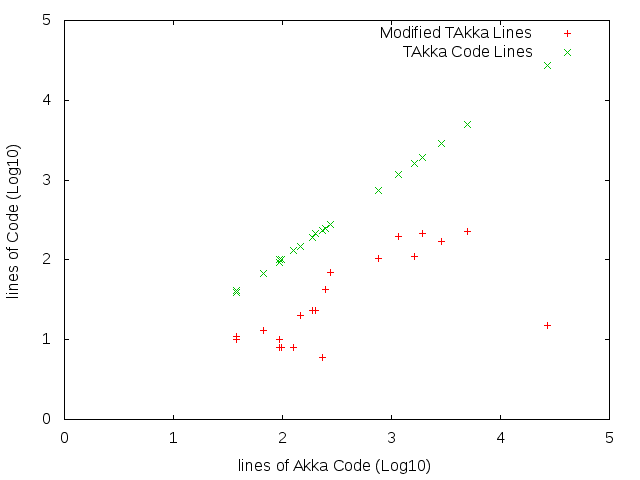
\includegraphics[scale=0.32]{Expressiveness/Expressiveness1.png}
        }
        \subfigure[Code Size: Relative Lines]{
           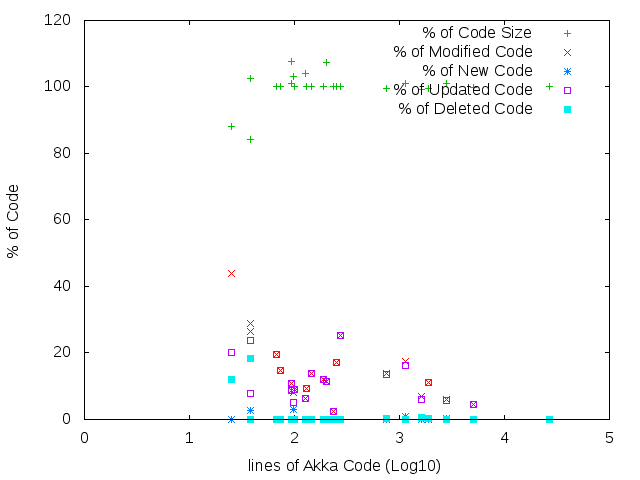
\includegraphics[scale=0.32]{Expressiveness/Expressiveness2.png}
        }
    \end{center}
    \caption{Code Size Evaluation}
   \label{fig:expressiveness}
\vspace{-10pt}   
\end{figure*}



\begin{figure*}[!ht]
     \begin{center}
        \subfigure[Throughput: Play]{
            \label{fig:play_throughput}
            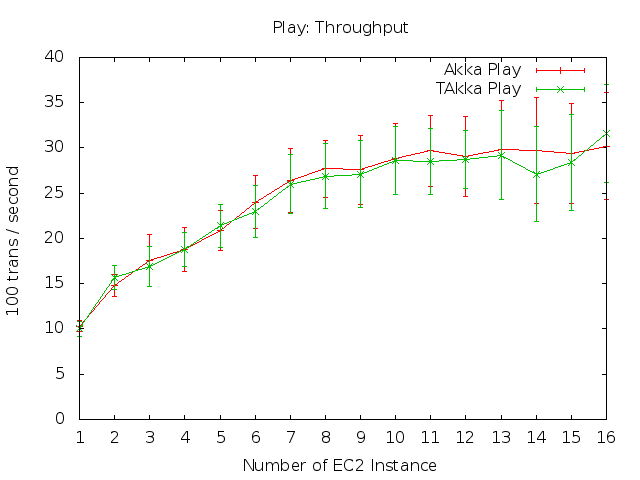
\includegraphics[scale=0.32]{TAkkaThroughput/Play_throughput.png}
        }
        \subfigure[Throughput: Socko]{
           \label{fig:socko_throughput}
           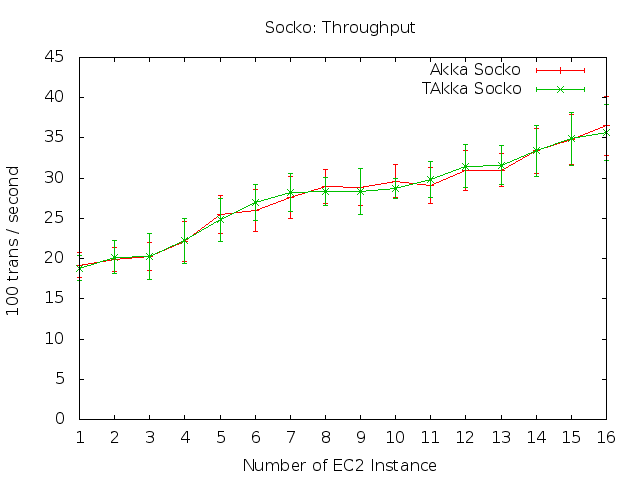
\includegraphics[scale=0.32]{TAkkaThroughput/Socko_throughput.png}
        }
    \end{center}
     \caption{Throughput Benchmarks}
   \label{throughput}
   \vspace{-10pt}
\end{figure*}

\begin{figure*}[!ht]
     \begin{center}
        \subfigure[Bang]{
            \label{fig:2_1}
            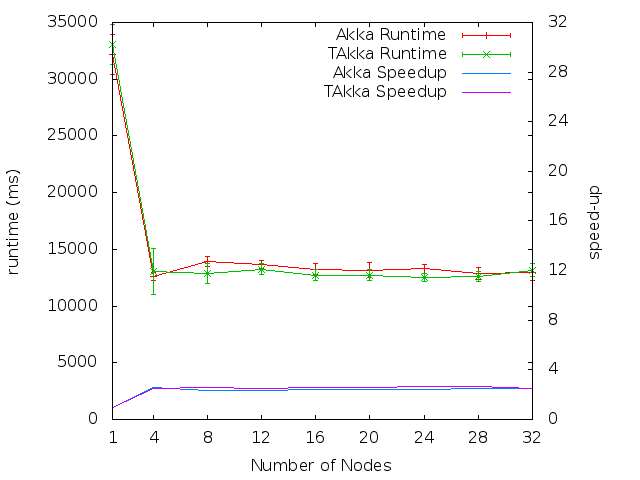
\includegraphics[scale=0.25]{efficiency/Bang.png}
        }
        \subfigure[Big]{
           \label{fig:2_2}
           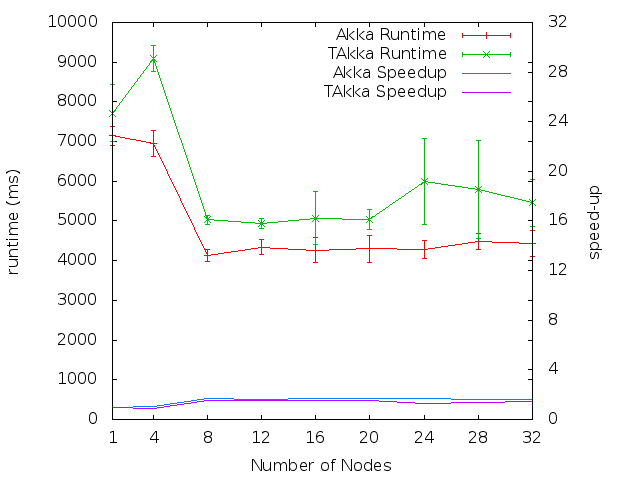
\includegraphics[scale=0.25]{efficiency/Big.png}
        }
        \subfigure[EHB]{
            \label{fig:2_3}
            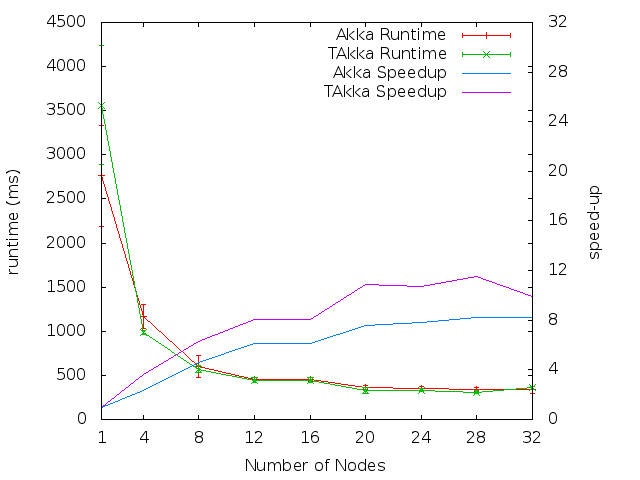
\includegraphics[scale=0.25]{efficiency/EHB.png}
        }\\
        \subfigure[MBrot]{
            \label{fig:2_5}
            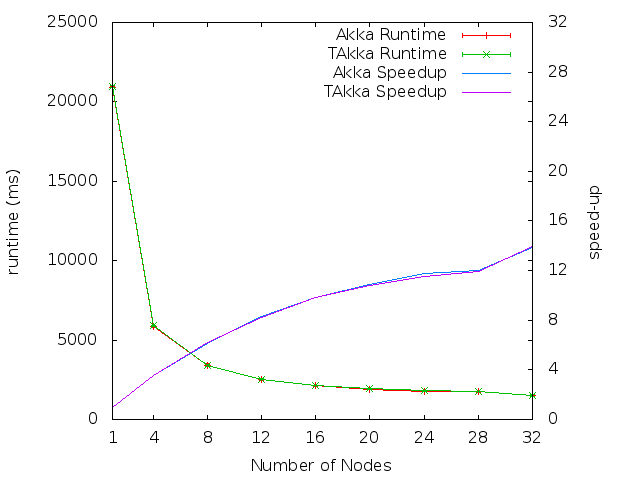
\includegraphics[scale=0.25]{efficiency/MBrot.png}
        }
        \subfigure[RAN]{
            \label{fig:2_7}
            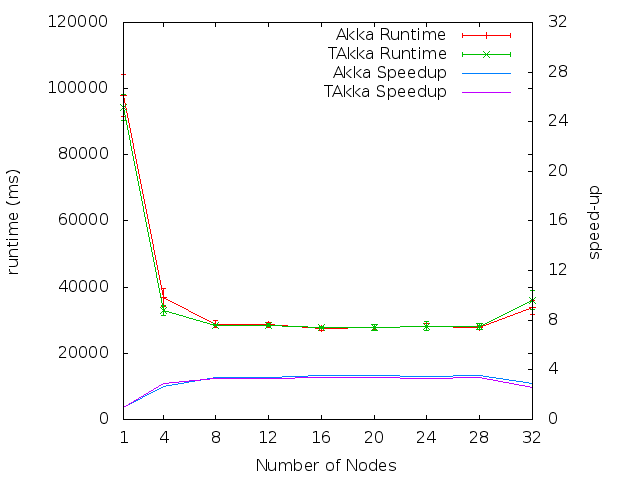
\includegraphics[scale=0.25]{efficiency/RAN.png}
        }
        \subfigure[SerialMsg]{
           \label{fig:2_8}
           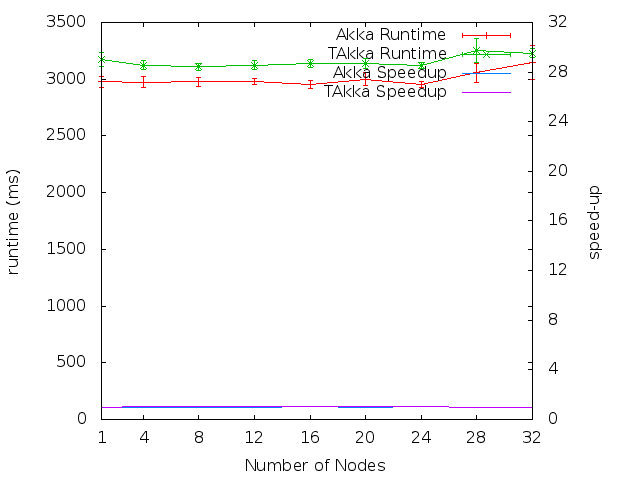
\includegraphics[scale=0.25]{efficiency/SerialMsg.png}
        }\\
    \end{center}
    \caption{Runtime \& Scalability Benchmarks}
   \label{runtime}
   \vspace{-10pt}
\end{figure*}

This section investigates whether the type discipline enforced by TAkka restricts the 
expressibility of Akka.  Table~\ref{express} lists the examples used for expressiveness checks.  
Examples are selected from Quviq \citep{quviq}
and open source Akka projects to ensure that the main requirements for actor 
programming are not unintentionally neglected.  Examples from 
Quviq are re-implemented using both Akka and TAkka.  Examples from 
Akka projects are re-implemented using TAkka.  Following standard practice,  
we assess the overall code modification and code 
size by calculating the geometric mean of all examples \citep{HePa06}. The evaluation results 
in Table~\ref{express} show that when porting an Akka program to TAkka, about 
8.5\% lines of code need to be modified including additional type declarations. 
Sometimes, the code size can be smaller because TAkka code does not 
need to handle unexpected messages.  On average, the total program size 
of Akka and TAkka applications are almost the same.  Figure~\ref{fig:expressiveness}
reports the same result in a Scatter chart.

A type error is reported by the compiler when porting the Socko example 
\citep{SOCKO} from its Akka implementation to its equivalent TAkka 
implementation. Socko is a library for building event-driven web services.  The 
Socko designer defines a {\tt SockoEvent} class to be the supertype of all 
events.  One subtype of {\tt SockoEvent} is {\tt HttpRequestEvent}, 
representing events generated when an HTTP request is received. The designer 
further implements subclasses of the {\tt Method} class, whose {\tt unapply} 
method is intended to have an output of type {\tt Option[HttpRequestEvent]}.  
The Socko designer made a type error in the method declaration so that the {\tt 
unapply} has output type {\tt Option[SockoEvent]}. The type error is not 
exposed in test examples because those examples only test HTTP events. 
The design flaw is exposed when rewriting Socko using TAkka.



% \vspace{-5pt}
\section{Throughput and Scalability}
\label{efficiency}
This section investigates whether managing type information in TAkka reduces
performance.  The TAkka library is built on Akka so that code for shared features 
can be re-used.  The three main sources of overheads in the TAkka implementation
are: (i) the cost of adding an additional operational layer on top of Akka 
code, (ii) the cost of constructing type descriptors, and (iii) the cost of 
transmitting type descriptors in distributed settings. We assess the effects of
the above overheads in terms of throughput and scalability.

The example used in the throughput benchmark is the JSON serialization example 
\citep{techempower}.  The example was implemented using Akka Play, TAkka Play, Akka 
Socko, and TAkka Socko.  All four versions of the web service are deployed to 
Amazon EC2 Micro instances (t1.micro), each of which has 0.615GB memory. The throughput 
is tested with up to 16 EC2 Micro instances.  For each number of EC2 instances, 
10 rounds of throughput measurement are executed to gather the average and 
standard deviation of the throughput. The results reported in Figure~\ref{throughput} show that web servers built using the Akka-based library and 
the TAkka-based library have very similar throughput.


We further investigate the speed-up of multi-node TAkka applications by 
porting 6  BenchErl benchmarks \citep{RELEASE} which do not involve Erlang/OTP 
specific features.  Each BenchErl benchmark spawns one master process and 
many child processes for a given task.  Each child process performs 
a certain amount of computation and reports the result to the master process.  
The benchmarks are run on a 32 node Beowulf cluster at Heriot-Watt 
University. Each Beowulf node comprises eight Intel 5506 cores running at
2.13GHz. All machines run under Linux CentOS 5.5. The Beowulf nodes are
connected with a Baystack 5510-48T switch.

Figures \ref{runtime} reports the results of the BenchErl 
benchmarks.   We report the average and the standard deviation 
of the run-time of each example.  Depending on the ratio of the computation 
time and the I/O time, benchmark examples scale at different levels.  In 
all examples, TAkka and Akka implementations have almost identical 
run-time and scalability.

In the BenchErl examples, child processes are asked to 
execute the same computation a number of times.  In contrast, distributed and 
cluster computing techniques are often used to solve a computationally 
expensive task by distributing sub-tasks to independent nodes.  To simulate 
such a scenario, another benchmark, N-Queens Puzzle \citep{wiki:nqueens}, is added. 
Finding all solutions of an N-Queen Puzzle is an NP-hard problem.  Therefore, a 
suitable $n$ makes the problem a good benchmark to demonstrate the advantage of 
cluster and distributed programming.  Figure~\ref{nqueens_efficiency}
reports the result when $n$ is set to $14$.  The result shows that both the Akka and 
TAkka implementation have good scalability and similar efficiency.


\begin{figure}[!h]
     \begin{center}
        \subfigure[N-Queens Time]{
            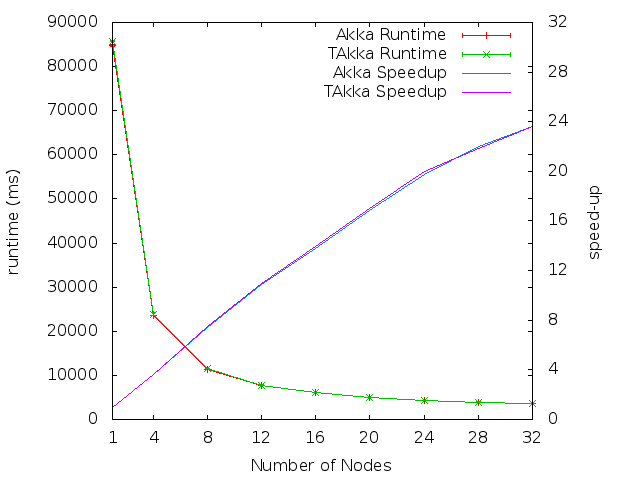
\includegraphics[scale=0.26]{efficiency/NQueens.png}
        }
    \end{center}
    \caption{Benchmark: N-Queens Puzzle}
   \label{nqueens_efficiency}
   \vspace{-10pt}
\end{figure}


\section{Conclusion}
\label{conclusion}

The Akka library accepts dynamically typed messages.  The TAkka
library introduces a type-parameter for actor-related classes. The additional 
type-parameter specifies the communication interface of 
that actor.  With the help of type-parameterized actors, unexpected 
messages to actors are rejected at compile time.
% In addition to eliminating programming bugs and type errors, 
% programmers would like to have a failure recovery mechanism for
% unexpected run-time errors.  
We have shown that type-parameterized 
actors can form supervision trees in the same way as untyped actors (Section~\ref{takka_design}).
We have shown that
adding type parameter does not restrict expressiveness, and requires
only small amounts of refactoring (Section~\ref{expressiveness}).  We have
shown that TAkka does not introduced performance penalties (Section~\ref{efficiency}), 
with respect to throughput, efficiency, and scalability.  The above results are encouraging for the 
use of types and supervision trees to implement reliable applications and improve the 
reliability of legacy applications with little effort.  
% We expect similar 
% results can be obtained in other actor libraries.

% \input{mainbody2}

% \section{Project Description}

\subsection{Background and Motivation}

Concurrent programming is facing new challenges due to the recent advent of multi-core processors, which rely on parallelism, and the pervasive demands of web applications, which rely on distribution.  Theoretic works on concurrency can be traced back to Petri net and other approaches invented in 1960s \cite{historyPA}.  Since 1980, more attention has been paid to the study of process calculi (a.k.a. process algebras), which provide a family of formal models for describing and reasoning about concurrent systems \cite{abramsky}.  The proliferation of Process Calculi marks the advance in concurrency theory.  ``The Dreams of Final Theories'' \cite{abramsky} for concurrency, however, have not been achieved.

In practice, it is difficult to build a reliable distributed system because of its complexity.  Firstly, a distributed system shares features and problems with other concurrent systems.  For instance, it is non-deterministic so that traditional input-output semantics is inadequate to be used for reasoning about its behaviour.  Secondly, scalability of a distributed system is usually a challenge for its developers.  For example, developers of a distributed system are unlikely to know the structure of the system in advance.  Moreover, the mobility \cite{MobileAmbients} of a distributed system requires the capability of changing its topological structure on the fly.  In addition, the latency of communication could be affected by many unpredictable factors.  Thirdly, the system should be tolerant of partial failures.  For example, when a site fails to respond to messages,  the system should address this failure by invoking a recovery mechanism.   	

Fortunately, some recent works provide a solid basis for the design of distributed programming languages.  For example, the ambient calculus \cite{MobileAmbients} models the movement of processes and devices.  Bigraphs \cite{bigraph_book}, a more abstract model, is aiming at describing spatial aspects and mobility of ubiquitous computing.  Session types \cite{Honda93typesfor, Honda_languageprimitives} guarantees that two parties of a session always communicate in a dual pattern.  Lastly, the join-calculus \cite{full_join} is a remarkable calculus which models features of distributed programming as well as provides a convenient construct, the join patterns, for resources synchronisation.  It is also important to note that the syntax of the join-calculus is close to a real programming language and therefore reduces the barrier between understanding the mathematical model and employing this abstract model to guide programming practices.

In addition, good programming principles, such as the OTP design principles\footnote{OTP is stand for Open Telecom Platform.  It provides a set of libraries for developing Erlang applications.  For the above reason, it is also known as Erlang/OTP design principles}, have been developed and verified by the long-term implementation practice.  OTP is a platform for developing concurrent, distributed, fault tolerant, and non-stop Erlang applications \cite{Erlang}.  In the past 20 years, the Erlang language was used to build large reliable applications like RabbitMQ, Twitterfall, and many telecommunications systems.

Nevertheless, Erlang is an untyped functional programming language whereas a typed language detects certain forms of data misuse earlier.  Therefore, it would be pleasant to combine advantages of static typing and OTP principles.  At the time of this writing, this idea has been partly realised in the akka framework \cite{akka}.  In spite of some attempts, the akka framework inherits some limitations of using untyped actors from the Erlang programming language.  This situation left us research potentials in this line.

\subsection{Project Aim}
\label{aim}
The aim of this project is to {\it{build a library that supports OTP design principles in a typed setting}}. The project intends to explore factors that encourage programmers to employ good programming principles.  This project will demonstrate how types and appropriate models help the construction of reliable distributed systems.

\subsection{Project Objectives}
\label{objectives}

\begin{enumerate}
  \item To identify a number of medium-sized applications implemented in Erlang using OTP principles.  Those examples will be served as references to evaluate frameworks that support OTP principles.  Candidate examples shall cover a wide range of aspects in distributed programming, including but not limited to 
    \begin{inparaenum} [(a)]
      \item transmitting messages and potentially computation closures, 
      \item modular composition of distributed components, 
      \item default and extensible failure recovery mechanism, 
      \item eventually consistency model for shared states, and 
      \item dynamic topology configuration and hot code swapping.
    \end{inparaenum} 
  \item To re-implement and compare identified applications within existing frameworks.  The primitives purpose of this work is to be aware of prominent features and limitations of existing frameworks.  As a research which contains certain level of overlaps with other existing and evolving frameworks, this research should distinguish itself from others by devised solutions to some problems which are difficulty to be solved by alternatives.  Moreover, the evaluation component formalised in this work is likely to be novel for comparing frameworks aiming at supporting distributed computation.  The same evaluation component will be used for evaluating our later developed library as well.
  \item To implement a library that supports OTP design principles in a typed setting.  The library could be built either on top of existing frameworks or with lower level constructs.  It important to note that the library might be based on an abstraction that is more general than the actor model.  Although OTP design principles were proposed for the Erlang language, which is based on the Actor model, we believe that it should be possible to rephrase those good programming principles in other models.  To demonstrate the wide applications of OTP design principles, the library interface should provide a certain level of generality so that it could be implemented by and used within different models.
  \item To demonstrate how the proposed library meets the demands of distributed programming.  At this stage, the proposed library will be used to (a) demonstrate how to write small programs aiming at different requirements; (b) demonstrate its scalability of programming in the large by reimplementing applications used in objective 1 and 2.
  \item To summarise some challenges in distributed programming and how to get around those difficulties with the proposed library and other programming frameworks.  The summary will reveal how language libraries, which is used for practical purposes, are related to their theoretical guidance underneath.  It may also plot research blanks for future study.
\end{enumerate}



% \section{Actor Programming}
\label{background}

\subsection{Actor Model and OTP Design Principles}

The Actor model defined by Hewitt et al.  \cite{Hewitt:1973} treats actors as
primitive computational components.  Actors collaborate by sending asynchronous
messages to each other.  An actor independently determines its reaction to
messages it receives.

The Actor model is adopted by the Erlang programming language, whose 
developers later summarized 5 OTP design principles to improve the 
reliability of Erlang applications \cite{OTP}.  We notice that the Behaviour 
principle, the Application principle, and the Release principle coincide with 
3 Java and Scala Programming practices listed in Table \ref{otp}.  The 
Release Handling principle requires runtime support for hot swapping.  In a 
platform where hot swapping is not supported in general, e.g. Java Virtual 
Machine (JVM), hot swapping a particular component can be simulated by updating 
the reference to that component. For example, Section \ref{hot_swapping} 
explains how to hot swap the behaviour of an actor in TAkka, which runs on the 
JVM. The Supervision principle, which is the central topic of this paper, 
has no direct correspondence in native JVM based systems.

\begin{table}[t]
\label{otp}
% \tbl{Implementing OTP Design Principles in an OO Language}{
 \begin{center}
\begin{tabular}{| l | p{4.5 cm} | }
\hline
  OTP Design Principle & JAVA/Scala Programming \\
\hline
  Behaviour & defining an abstract class \\
\hline
  Application  & defining an abstract class that has two abstract methods: start and stop \\
\hline
  Release  & packaging related application classes  \\ 
\hline
  Release Handling  & hot swapping support on key modules is required \\
\hline
  Supervision  & no direct correspondence  \\
\hline
\end{tabular}
 \caption[]{Using OTP Design Principles in JAVA/Scala\\  Programming}
\end{center}
%}
\end{table}




\subsection{Akka Actor}
\label{akka actor}


An Akka Actor has four essential components as shown in Figure 
\ref{fig:akka_actor_api}: (i) a receive function that defines its reaction to 
incoming messages, (ii) an actor reference pointing to  itself, (iii) the actor 
 context representing the outside world of the actor, and (iv) the supervisor 
strategy for its children.

\begin{figure}[h]
\label{fig:akka_actor_api}
\begin{lstlisting}[language=scala]
package akka.actor
trait Actor{
  def receive:Any=>Unit
  val self:ActorRef
  val context:ActorContext
  var supervisorStrategy: SupervisorStrategy
}
\end{lstlisting}
\caption{Akka Actor API}
\end{figure}

Figure \ref{akkastring} shows an example actor in Akka.  The {\tt receive} 
function of the Akka actor has type {\tt Any$\Rightarrow$Unit} but the 
defined actor, {\tt ServerActor}, is only intended to process strings.  At Line 
16, a {\tt Props}, an abstraction of actor creation, is initialized and passed 
to an actor system, which creates an actor with name \textcolor{mauve}{\tt 
server} and returns a reference pointing to that actor.  Another way to obtain 
an actor is using the {\tt actorFor} method as shown in line 24.  We then use 
actor references to send the actor string messages and integer messages.  
String messages are processed in the way defined by the receive function.

\begin{figure}[t]
 \label{akkastring}
      \begin{lstlisting}[language=scala]
class ServerActor extends Actor {
  def receive = {
    case m:String => println("received message: "+m)
  }
}

class MessageHandler(system: ActorSystem) extends Actor {
  def receive = {
    case akka.actor.UnhandledMessage(message, sender, recipient) =>
      println("unhandled message:"+message);
  }
}

object ServerTest extends App {
  val system = ActorSystem("ServerTest")
  val server = system.actorOf(Props[ServerActor], "server")
  
  val handler = system.actorOf(Props(new MessageHandler(system)))
  system.eventStream.subscribe(handler,
                     classOf[akka.actor.UnhandledMessage]);
  server ! "Hello World"
  server ! 3
  
  val serverRef = system.actorFor("akka://ServerTest/user/server")
  serverRef ! "Hello World"
  serverRef ! 3
}


/*
Terminal output:
received message: Hello World
unhandled message:3
received message: Hello World
unhandled message:3
*/
    \end{lstlisting}
    \caption{A String Processor in Akka}
\end{figure}

Undefined messages are treated differently in different actor libraries.  In
Erlang, an actor keeps undefined messages in its mailbox, attempts to process
the message again when a new message handler is in use.  In versions prior to
2.0, an Akka actor raises an exception when it processes an undefined message.
In recent Akka versions, an undefined message is discarded by the actor and an
{\tt UnhandledMessage} event is pushed to the event stream of the actor system.
The event stream may be subscribed by other actors who are interested in
particular event messages.  To handle the unexpected integer message in the
above short example, an event handler is defined and created with 6 lines of 
code.


\subsection{Supervision}
\label{akkasup}



Reliable Erlang applications typically adopt the Supervision Principle
 \cite{OTP}, which suggests that actors should be organized in a tree structure 
so that any failed actor can be properly restarted by its supervisor.  
Nevertheless, adopting the Supervision principle is optional in Erlang.

The Akka library makes supervision obligatory by restricting the way of 
creating actors. Actors can only be initialized by using the {\tt actorOf}
method provided by {\tt ActorSystem} or {\tt ActorContext}.  Each actor system
provides a guardian actor for all user-created actors.  Calling the {\tt
actorOf} method of an actor system creates an actor supervised by the 
guardian actor.  Calling the {\tt actorOf} method of an actor context 
creates a child actor supervised by that actor.  Therefore, all user-created  
actors in an actor system, together with the guardian actor of that actor 
system, form a tree structure.  Obligatory supervision unifies the 
structure of actor deployment and simplifies the work of system maintenance.

Each actor in Akka is associated with an actor path.  The string representation
of the actor path of a guardian actor has format 
{\it akka://mysystem@IP:port/user}, where {\it mysystem} is the name of the 
actor system, {\it IP} and {\it port} are the IP address and the 
port number which the actor system listens to, and {\it user} is the name of 
the guardian actor.  The actor path of a child actor is actor path of its 
supervisor appended by the name of the child actor, either a user specified 
name or a system generated name.

Figure \ref{supervisedcalculator} defines a simple calculator which supports
multiplication and division. The simple calculator does not consider the
problematic case of dividing a number by 0, where an {\tt
ArithmeticException} will be raised.  We then define a safe calculator as the 
supervisor of the simple calculator.  The safe calculator delegates 
calculation tasks to the simple calculator and restarts the simple calculator 
when an {\tt ArithmeticException} is raised.  The supervisor strategy of
the safe calculator also specifies the maximum number of failures its child may 
have within a given time range.  If the child fails more frequently than the 
allowed frequency, the safe calculator will be  stopped, and its failure will be
reported to its supervisor, the system guardian actor in this example.  The
terminal output shows that the simple calculator is restarted before the third 
message and the fifth message are delivered.  The last message is not processed
because both calculators are terminated since the simple calculator fails more 
frequently than allowed.

\begin{figure}
\label{supervisedcalculator}

  \begin{lstlisting}[language=scala]
case class Multiplication(m:Int, n:Int)
case class Division(m:Int, n:Int)

class Calculator extends Actor {
  def receive = {
    case Multiplication(m:Int, n:Int) =>
      println(m +" * "+ n +" = "+ (m*n))
    case Division(m:Int, n:Int) =>
      println(m +" / "+ n +" = "+ (m/n))
  }
}

class SafeCalculator extends Actor {
  override val supervisorStrategy =
    OneForOneStrategy(maxNrOfRetries = 2, withinTimeRange = 1 minute) {
      case _: ArithmeticException  =>
        println("ArithmeticException Raised to: "+self)
        Restart
    }
  val child:ActorRef = context.actorOf(Props[Calculator], "child")
  def receive = {
    case m => child ! m
  }
}

  val system = ActorSystem("MySystem")
  val actorRef:ActorRef = system.actorOf(Props[SafeCalculator],
"safecalculator")

  calculator ! Multiplication(3, 1)
  calculator ! Division(10, 0)
  calculator ! Division(10, 5)
  calculator ! Division(10, 0)
  calculator ! Multiplication(3, 2)
  calculator ! Division(10, 0)
  calculator ! Multiplication(3, 3)

/*
Terminal Output:
3 * 1 = 3
java.lang.ArithmeticException: / by zero
ArithmeticException Raised to: Actor[akka://MySystem/user/safecalculator]

10 / 5 = 2
java.lang.ArithmeticException: / by zero
ArithmeticException Raised to: Actor[akka://MySystem/user/safecalculator]
java.lang.ArithmeticException: / by zero

3 * 2 = 6
ArithmeticException Raised to: Actor[akka://MySystem/user/safecalculator]
java.lang.ArithmeticException: / by zero
*/
    \end{lstlisting}
  \caption{Supervised Calculator}
\end{figure}
% \section{Mixing Static and Dynamic Type Checking}
\label{type_checking}
A key advantages of static typing is that it detects some type errors at an 
early stage, i.e., at compile time.  The TAkka library is designed to detect 
type errors as early as possible.  Nevertheless, not all type errors can be 
statically detected, and some dynamic type checks are required. To address this 
issue, a notion of run-time type descriptor is required.  This section 
summarizes the type reflection mechanism in Scala and  explains
how it benefits the implementation of our typed name
server.  Our typed name server can be straightforwardly ported
to other platforms that support type reflection.

\subsection{Scala Type Descriptors}

As in Java, generic types are erased by the Scala compiler.
To record type information that is required at runtime but might be
erased, Scala users can ask the compiler to keep the type information
by using the {\tt Manifest} class. The Scala standard library contains four
manifest classes as shown in Figure \ref{scala_api_manifest}.
A {\tt Manifest[T]} encapsulates the runtime type representation 
of some type {\tt T}.   {\tt Manifest[T]} a subtype of {\tt ClassManifest[T]}, 
which declares methods for subtype ($<:<$) test and supertest ($>:>$).  
The object {\tt NoManifest} represents type information that is required
by a paraterized type but is not available in scope.  {\tt OptManifest[+T]} is 
the supertype of {\tt ClassManifest[T]} and {\tt OptManifest}.

\begin{figure}[!h]
\begin{lstlisting}[language=scala, escapechar=?]
package scala.reflect
trait OptManifest[+T] extends Serializable
object NoManifest extends OptManifest[Nothing] with Serializable
trait Manifest[T] extends ClassManifest[T] with Serializable
trait ClassManifest[T] extends OptManifest[T] with Serializable
  def <:<(that: ClassManifest[_]): Boolean
  def >:>(that: ClassManifest[_]): Boolean
  erasure: Class[_]
\end{lstlisting}
\caption{Scala API: Manifest Type Hierarchy}
\label{scala_api_manifest}
\end{figure}

\begin{comment}
\subsection{Scala Type Descriptors}
Scala 2.8 defines a {\tt Manifest} class whose instance is a serializable 
first class type descriptor used at runtime.  With the help of 
the {\tt Manifest} class, users can record the type information, including 
generic types, which may be erased by the Java compiler.  

In the Scala interactive session below, we obtain a Manifest value at Line 5 and 
test a subtype relationship at Line 8.  To define a method that obtains type 
information of a generic type, Scala requires a type tag as an implicit 
argument to the method.  To simplify the API, Scala further provides a form of
syntactic sugar called context bounds.  We define a method using context
bounds at Line 11, which is compiled to the version using implicit 
arguments as shown at Line 12.


\begin{lstlisting}
scala> class Sup; class Sub extends Sup
defined class Sup
defined class Sub

scala> manifest[Sub]
res0: Manifest[Sub] = Sub

scala> manifest[Sub] <:< manifest[Sup]
res1: Boolean = true

scala> def getType[T:Manifest] = {manifest[T]}
getType: [T](implicit evidence$1: Manifest[T])Manifest[T]

scala> getType[Sub => Sup => Int]
res2: Manifest[Sub => (Sup => Int)] = scala.Function1[Sub, scala.Function1[Sup, Int]]

\end{lstlisting}

 
\end{comment}

\begin{figure}[!h]
\label{tsymbol}
\begin{lstlisting}
case class TSymbol[T:Manifest](val s:Symbol) {
    private [takka] val t:Manifest[_] = manifest[T]
    override def hashCode():Int = s.hashCode()  
}
case class TValue[T:Manifest](val value:T){
  private [takka] val t:Manifest[_] = manifest[T]
}
\end{lstlisting}
\caption{TSymbol and TValue}
\end{figure}

\subsection{Typed Name Server}
\label{nameserver}

In distributed systems, a name server maps each registered name, usually a
unique string, to a dynamically typed value, and provides a function to look up 
a value for a
given name. A name can be encoded as a {\tt Symbol} in Scala so that names
which represent the same string have the same value.  As a value retrieved from 
a name server is {\it dynamically typed}, it needs to be checked against and be 
cast to the expected type at the client side before using it.
To overcome the limitations of the untyped name server, we design and implement
a typed name server which maps each registered typed name to a value of the
corresponding type, and allows to look up a value by giving a typed name.

A typed name, {\tt TSymbol}, is a name shipped with a type descriptor.  A 
typed value, {\tt TValue}, is a value shipped with a type descriptor, which
describes a super type of the most precise type of that value.  
In Scala, {\tt TSymbol} and {\tt TValue} can be simply defined as in Figure
\ref{tsymbol}.  {\tt TSymbol} is declared as a {\it case class} in Scala so 
that it can be used as a data constructor and for pattern matching.  In 
addition, the type descriptor, {\tt t}, is constructed automatically and is 
private to the {\tt takka} package so that only it can only be accessed by TAkka 
library developers. {\tt TValue} is implemented similarly for the same reason.

With the help of {\tt TSymbol}, {\tt TValue}, and a hashmap, a typed name 
server provides the following three operations:




\begin{itemize}
  \item {\tt set[T:Manifest](name:TSymbol[T], value:T):Boolean}

The {\tt set} operation registers a typed name with a value of corresponding 
type and returns true if the symbolic representation of {\it name} has {\it 
not} been registered; otherwise the typed name server discards the request and
returns false.

  \item {\tt unset[T](name:TSymbol[T]):Boolean}

The {\tt unset} operation removes the entry {\it name} and returns true if (i) 
its symbolic representation is registered and (ii) the type {\tt T} is a 
supertype of the registered type; otherwise the operation returns false.

  \item {\tt get[T] (name: TSymbol[T]): Option[T]}

The {\tt get} operation returns Some(v:{\tt T}), where {\tt v} is the value 
associated with {\it name}, if (i) {\it name} is a registered name and (ii) 
{\tt T} is a supertype of the registered type; otherwise the operation returns 
None.

\end{itemize}

Notice that {\tt unset} and {\tt get} operations succeed as long as the 
associated type of the input name is the supertype of the associated type of 
the registered name.  To permit polymorphism, the {\tt hashcode} method of {\tt 
TSymbol} defined in  Figure {\ref{tsymbol}} does not take type values into 
account.  Equivalence comparison on {\tt TSymbol} instances, however, should 
consider the type.  Although the {\tt TValue} class does not appear in the
APIs for library users, it is required for an efficient library implementation 
because the type 
information in {\tt TSymbol} is ignored in the hashmap.  Overriding the
hash function of {\tt TSymbol} also prevents the case where users accidentally
register two typed names with the same symbol but different types,
in which case if one type is a supertype of the other, the return value of
{\tt get} may be non-deterministic.  Last but not least, when an operation 
fails, the name server returns {\tt false} or {\tt None} rather than raising an
exception so that the name server is always available.

In general, dynamic type checking can be carried out in two ways.  The first 
method is to check whether the most precise type of a value conforms to the
structure of a data type.  Examples of this method include dynamically typed
languages and the {\tt instanceof} method in Java and other languages.  The
second method is to compare two type descriptors at run time.  The
implementation of our typed name server employs the second method because  
it detects type errors which may otherwise be left out.  Our
implementation requires the runtime type reification feature provided by Scala.
In a system that does not support type reification, implementing typed name 
server can be difficult.



% \section{Adding Type Parameter to Actor Library}

This section examines actor programming in the Akka library and how type parameters are added to actor-related classes to improve type safety.  We show that supervision trees in TAkka are constructed in the same way as in Akka.  This section concludes with a brief discussion about alternative designs used by Akka and other actor libraries.

\mycomment{Explain Actor Programming.  Compare Akka and TAkka side by side.}

\subsection{The Actor Class}

An Actor has four important fields given in Figure-\ref{actor_api}:
(i) a receive function that defines its reaction to incoming messages, (ii)
an actor reference pointing to  itself, (iii) the actor  context representing
the outside world of the actor, and (iv) the supervisor strategy for its
children.


An TAkka {\bf Actor} has Akka equivalent fields as shown in
Table \ref{actor_api}.  Different from other actor libraries, every TAkka
actor class takes a type parameter {\bf M} which specifies the type of messages
it expects to receive.  The same type parameter is used as the input type of the
receive function, the type parameter of actor context and the type parameter of
the actor reference pointing to itself.  We introduce a new field $mt$ to inform the compiler that the type parameter of the {\bf Actor} class should be recorded.

\begin{table}[h]
\label{actor_api}
\caption{Akka and TAkka Actor}
%  \begin{adjustwidth}{-1.8cm}{}
  \begin{tabular}{ l   l }
\begin{lstlisting}[language=scala]
package akka.actor
trait Actor {

  def typedReceive:Any=>Unit
  val typedSelf:ActorRef
  val typedContext:ActorContext
  var supervisorStrategy:
         SupervisorStrategy
}
\end{lstlisting} &
\begin{lstlisting}[language=scala]
package takka.actor
trait Actor[M] {
  implicit val mt : TypeTag[M]
  def typedReceive:M=>Unit
  val typedSelf:ActorRef[M]
  val typedContext:ActorContext[M]
  var supervisorStrategy: 
         SupervisorStrategy
}
\end{lstlisting}
  \end{tabular}
%  \end{adjustwidth}
\end{table}



The three immutable fields of TAkka {\bf Actor}: {\it mt}, {\it typedContext} and {\it
typedSelf}, will be initialised automatically when the actor is created.
Application developers may override the default supervisor strategy in the way
explained in \S\ref{supervision}.  The implementation of the {\it typedReceive}
method, on the other hand, is left to developers.


\subsection{Actor Reference}
\label{actor_ref}
A reference pointing to an Actor of type {\bf Actor[M]} has type {\bf ActorRef[M]}.  It provides a {\it !} method, through which users could send a message of type {\bf M} to the referenced actor.  Sending an actor reference a message whose type is not the
expected type will raise a compile error.  By using type-parametrized actor
references, the receiver does not need to worry about unexpected messages while
senders can ensure that messages will be understood and processed, as long as
the message is delivered.

In a type system which supports polymorphism, {\bf ActorRef} should be
contravariant.  We further provide a {\it publishAs} method which type-safely
casts an actor reference to a version of its supertype.  In another word, the
output actor reference accepts partial forms of messages that are accepted by
the input actor reference.  The ability of publishing partial services makes
TAkka a good tool for solving security problems such as the type pollution
problem described at \S\ref{type_pollution}.

\begin{table}[h]
\label{ActorRef}
  \begin{tabular}{ l  l }
      \begin{lstlisting}[language=scala]
abstract class ActorRef {

  def !(message: Any):Unit
  
  
}
    \end{lstlisting} 
    &
    \begin{lstlisting}[language=scala]
abstract class ActorRef[-M]
    (implicit mt:TypeTag[M]) {
  def !(message: M):Unit
  def publishAs[SubM<:M]
      (implicit mt:TypeTag[SubM]):ActorRef[SubM]
}
    \end{lstlisting}     
  \end{tabular}
    \caption{Actor Reference}
\end{table}

The code below defines and uses a string processing actor in Akka and TAkka.  The receive
function of Akka Actor has type {\bf Any$\Rightarrow$Unit} but the defined actor
only intends to process strings. Both examples create an actor inside an actor system
and returns a reference pointing to that actor.  The same string message is sent to actor in both examples
and processed in the way defined in the receive function.  Sending an integer message, which is not expected
by both actors; However, is permitted in the Akka version but rejected by the TAkka version.

\begin{table}[h]
\label{ActorRef}
     \begin{adjustwidth}{-0.8cm}{}
  \begin{tabular}{ l   l }
      \begin{lstlisting}[language=scala]
class MyActor extends Actor {
  def receive:Any => Unit = {
    case m:String =>
      println("Received message: " + m)
  }
}

val system = ActorSystem("MySystem")
val actorRef:ActorRef =
    system.actorOf(Props[MyActor])
actorRef ! "Hello World!"
actorRef ! 3



/*
Terminal output:
Received message: Hello World!
*/
    \end{lstlisting}
&
      \begin{lstlisting}[language=scala]
class MyActor extends Actor[String] {
  def typedReceive:String=>Unit = {
    case m:String =>
      println("received message: "+m)
  }
}

val system = ActorSystem("MySystem")
val actorRef:ActorRef[String] = 
    system.actorOf(Props[String, MyActor])
actorRef ! "Hello World!"
// actorRef ! 3 
// compile error: type mismatch; found : Int(3)
//   required: String

/*
Terminal output:
Received message: Hello World!
*/
    \end{lstlisting}

  \end{tabular}
  \end{adjustwidth}
    \caption{A Actor String Processor}
\end{table}

Undefined messages are treated differently in different actor libraries.  In
Erlang, an actor keeps undefined messages in its mailbox, attempts to process
the message again when a new message handler is in use.  In versions prior to
2.0, an Akka actor raises an exception when it processes an undefined message.
In recent Akka versions, undefined message is discarded by the actor and an {\bf
UnhandledMessage} event is pushed to the event stream of the actor system. The
event stream may be subscribed by other actors to which all events will be
published.  In the example code no subscriber of the event stream is defined and
the integer message is simply discarded.


\subsection{Props and Actor Context}
\label{actor_context}
\mycomment{Explain Akka version and TAkka version at the same time}

A Props is the configuration of actor creation.  A Props of type {\bf Prop[M]}
specifies how to create an actor of type {\bf Actor[M]} and returns an actor
reference of type {\bf ActorRef[M]}.  A Prop should be created by one of
following APIs, where {\bf MyActor} should be a subtype of {\bf Actor[M]}:

\begin{table}[h]
\label{Props}
     \begin{adjustwidth}{-1.2cm}{}
  \begin{tabular}{ l  l }

\begin{lstlisting}[language=scala]
 val props:Props = Props[MyActor]
 val props:Props = Props(new MyActor)
 val props:Props = Props(myActor.getClass)
\end{lstlisting}
&
\begin{lstlisting}[language=scala]
 val props:Props[M] = Props[M, MyActor]
 val props:Props[M] = Props[M](new MyActor)
 val props:Props[M] = Props[M](myActor.getClass)
\end{lstlisting}
  \end{tabular}
     \end{adjustwidth}
    \caption{Props Creation API}
\end{table}
  

Contrary to actor reference, an actor context describes the outside world of the
actor.   For security consideration, actor context is only available inside the
actor definition.  By using APIs in Figure \ref{ActorContext}, an actor can (i)
retrieving an actor reference according to a given actor path, (ii) creating a
child actor with system generated or user specified name, (iii) set a timeout
during which period a new message shall be received, and (iv) update its
behaviours.

The {\it ActorFor} method in the {\bf ActorContext} classes returns an actor
reference of the desired type, if the actor located at the specified actor path
has a compatible type.  To implement the {\it ActorFor} method, we would like to
have a more general mechanism that will return a value of the desired type
when the corresponding key is given.  To this end, we designed and implemented a
typed name server which will be explained \S\ref{nameserver}.

The {\it become} method enables hot code swap on the behaviour of an actor.  The
{\it become} method in TAkka is different from code swap in Akka in two aspects.
 Firstly, the supervision strategy could be updated as well.  Secondly, the new
receive function must be more general than the previous version.  As a result,
no stack of receive functions is required.  Interestingly, the implementation of
{\it become} involves a mix of static and dynamic type checks.  Details of the
implementation will be discussed in \S\ref{code_evolution}.

\begin{table}[h]
\label{ActorContext}
   \begin{adjustwidth}{-1.3cm}{}
  \begin{tabular}{ l   l }
      \begin{lstlisting}[language=scala]
trait ActorContext {
  def actorFor(actorPath:String):ActorRef
  
  def actorOf(props: Props):ActorRef
  def actorOf(props: Props, 
              name: String): ActorRef
  def setReceiveTimeout
             (timeout: Duration): Unit

  def become(
      newReceive: Any => Unit,
  ):ActorRef
}



    \end{lstlisting}
&
    \begin{lstlisting}[language=scala]
trait ActorContext[M] {
  def actorFor [Msg] (actorPath: String)
       (implicit mt: TypeTag[Msg]): ActorRef[Msg]
  def actorOf[Msg](props: Props[Msg])
        (implicit mt: TypeTag[Msg]): ActorRef[Msg]
  def actorOf[Msg](props: Props[Msg], name: String)
        (implicit mt: TypeTag[Msg]): ActorRef[Msg]
  def setReceiveTimeout(timeout: Duration): Unit

  def become[SupM >: M](
      newTypedReceive: SupM => Unit,
      newSystemMessageHandler:
                         SystemMessage => Unit,
      newSupervisionStrategy:SupervisionStrategy
  )(implicit smt:TypeTag[SupM]):ActorRef[SupM]
}
    \end{lstlisting}
    \end{tabular}
     \end{adjustwidth}
    \caption{Actor Context}
\end{table}


\subsection{Supervision Strategies}
\label{supervision}

There are three supervision strategies defined in Erlang/OTP: one-for-one,
one-for-all, and rest-for-one\cite{OTP}.  If a supervisor adopts the one-for-one
supervision strategy, a child will be restarted when it fails.  If a supervisor
adopts the one-for-all supervision strategy, all children will be restarted when
any of them fails.  In Erlang/OTP, children are started in a user-specified
order.  If a supervisor adopts the rest-for-one supervision strategy, all
children started after the failed child will be restarted.  For each
supervision strategy, users can further specify the maximum restarts of any
child within a period.

The Akka library only considers the one-for-one strategy and the one-for-all
strategy.  The rest-for-one strategy is not considered because children are not
created according to a user-specified order.  The default supervision strategy
is a one-for-one strategy that permits unlimited restarts.  Users can define
their own supervision strategy by using APIs given in Figure-\ref{super}.  {\bf
OneForOne} corresponds to the one-for-one strategy in Erlang whereas {\bf
OneForAll} corresponds to the all-for-one strategy in Erlang.  Both
strategies are constructed by providing required parameters.  {\bf Directive} is
an enumerable type whose value is {\bf Escalate}, {\bf Restart}, {\bf Resume},
or {\bf Stop}.  Notice that neither supervision strategies require any type-parametrized class. Therefore, both supervision strategies
are constructed in TAkka in the same way as in Akka.


\begin{figure}[h]
\label{super}
    \begin{lstlisting}    
abstract class SupervisorStrategy
case class OneForOne(restart:Int, time:Duration)
                    (decider: Throwable => Directive) extends SupervisorStrategy
case class OneForAll(restart:Int, time:Duration)
                    (decider: Throwable => Directive) extends SupervisorStrategy
    \end{lstlisting}
    \caption{Supervision Strategies}
\end{figure}


\subsection{Handling System Messages}

Actors are communicated with each other by sending messages.  To maintain a
supervision tree, for example to monitor and control the liveness of actors, a
special category of messages should be addressed by all actors.  We define a
trait {\bf SystemMessage} to be the supertype of all messages for system
maintenance purposes.  Based on the design of Erlang and Akka, we consider
following messages should be included in system messages:

\begin{itemize}
  \item {\bf ChildTerminated(child: ActorRef[M])}  

  a message sent from a child actor to its supervisor before it terminates.

  \item {\bf Kill}

  a message sent from a supervisor to its child.

  \item {\bf Restart}
 
  a message sent from a supervisor to its terminated child asking to restart the child.

  \item {\bf ReceiveTimeout}

  a message sent from an actor to itself when it did not receive any message after a timeout.

\end{itemize}

An open question is which system messages are allowed to be handled by users.
In Erlang and early Akka versions, all system messages could be explicitly
handled by users in the {\it receive} block.  In recent Akka versions, there is
a consideration that some system messages should be handled in library
implementation but not be handled by library users.

Considering that there are only two supervision strategies to consider, both of
which have clearly defined operational behaviours, all messages related to the
liveness of actors are handled in the TAkka library implementation.  General
library users may indirectly affect the system message handler via specifying
the supervision strategies.  On the contrary, messages related to the behaviour
of an actor, e.g. ReceiveTimeout, are better to be handled by application
developers.  In TAkka, {\bf ReceiveTimeout} is the only system message that can
be explicitly handled by users.

\subsection{Alternative Designs}
\label{alternative designs}


\paragraph{Akka Typed Actor}
In the Akka library, there is a special class called {\bf TypedActor}, which
contains an internal actor and could be supervised.  Users of typed actor invoke
a service by calling a method instead of sending messages.  The typed actor
prevents some type errors but has two limitations.  For one thing, typed actor
does not permit code evolution.  For the other, avoiding type pollution when
using typed actor would be as awkward as using a plain objected-oriented model.

\paragraph{Actors with or without Mutable States}
The actor model formalised by Hewitt et al. \cite{Hewitt:1973} does not specify
its implementation strategy.  In Erlang, a functional programming language,
actor does not have mutable states.  In Scala, an objected-oriented
programming language, actor may have mutable states.  The TAkka library is
built on top of Akka and implemented in Scala as well.  As a result, TAkka does
not prevent users from defining actors with mutable states.  Nevertheless, the
library designers would like to encourage using actors in a functional
style because actors with mutable states is difficult to synchronize in a
cluster environment.

In a cluster, resources are replicated at different locations to provide
efficient fault-tolerant services.  Known as the CAP theorem \cite{CAP}, it is
impossible to achieve consistency, availability, and partition tolerance in a
distributed system simultaneously.  For actors without mutable state, system
providers do not need to worry about consistency.  For actors that contain
mutable states, system providers have to either sacrifice availability or
partition tolerance, or modify the consistency model.  For example, Akka actor
has mutable states and Akka cluster employs an eventual consistency
model \cite{Kuhn12}.

\paragraph{Linked Actors}
Alternative to forming supervision trees, reliability of actor-based programs
could be improved by linking related actors \cite{ErlangWeb}. Linked actors are
aware of the death of each other.  Indeed, supervision tree is a special
structure for linking actors.  For this reason, we consider actor linking is a
redundant design in a system where supervision is obligatory.  After all, if
the computation of an actor relies on the liveness of another actor, those two
actors should be organised in the same logic supervision tree.






% \section{Evolution, Not Revolution }
\label{evolution}

Akka systems can be smoothly migrated to TAkka systems. In other words, 
existing systems can evolve to introduce more types, rather than requiring a 
revolution where all actors and interactions must be typed.

The above property is analogous to adding generics to Java programs.  Java 
generics are carefully designed so that programs without generic types can be 
partially replaced by an equivalent generic version (evolution), rather than 
requiring generic types everywhere (revolution) \citep{JGC}.

In previous sections, we have seen how to use Akka actors in an Akka 
system (Figure \ref{fig:akkastring}) and how to use TAkka actors in a TAkka 
system (Figure \ref{takkastring}).  In the following, we will explain how to 
use TAkka actors in an Akka system and how to use an Akka actor in a TAkka 
system.

\begin{figure}[!h]

      \begin{lstlisting}[language=scala, escapechar=?]
class TAkkaStringActor extends ?\textcolor{blue}{takka.actor.TypedActor[String]}? {
  def ?\textcolor{blue}{typedReceive}? = {
    case m:String => println("received message: "+m)
  }
}
class MessageHandler(system: akka.actor.ActorSystem) extends akka.actor.Actor {
  def receive = {
    case akka.actor.UnhandledMessage(message, sender, recipient) =>
      println("unhandled message:"+message);
  }
}
object TAkkaInAkka extends App {
  val akkasystem = akka.actor.ActorSystem("AkkaSystem")
  val akkaserver = akkasystem.actorOf(
    akka.actor.Props[TAkkaStringActor], "aserver")

  val handler = akkasystem.actorOf(
    akka.actor.Props(new MessageHandler(akkasystem)))
  
  akkasystem.eventStream.subscribe(handler,
     classOf[akka.actor.UnhandledMessage]);
  akkaserver ! "Hello Akka"
  akkaserver ! 3
  
  val takkasystem = ?\textcolor{blue}{takka}?.actor.ActorSystem("TAkkaSystem")
  val typedserver = takkasystem.actorOf(
     takka.actor.Props[?\textcolor{blue}{String,}? TAkkaStringActor], "tserver")
  
  val untypedserver = takkaserver.untypedRef
  
  takkasystem.system.eventStream.subscribe(
    handler,classOf[akka.actor.UnhandledMessage]);
  
  untypedserver ! "Hello TAkka"
  untypedserver ! 4
}
/*
Terminal output:
received message: Hello Akka
unhandled message:3
received message: Hello TAkka
unhandled message:4
*/
    \end{lstlisting}
    \caption{TAkka actor in Akka application}
\label{takkaINakka}    
\end{figure}

\subsection{TAkka actor in Akka system}

It is often the case that an actor-based library is implemented by one 
organization but used in a client application implemented by another 
organization.  If a developer decides to upgrade the library implementation 
using TAkka actors, for example, by upgrading the Socko Web Server 
\citep{SOCKO}, the Gatling \citep{Gatling} stress testing tool, or the core 
library of the Play framework \citep{play_doc}, as we do in Section 
\ref{expressiveness}, will the upgrade affect client code, especially 
legacy applications built using the Akka library?  Fortunately, TAkka actors and actor 
references are implemented using inheritance and delegation respectively so 
that no changes are required for legacy applications.

TAkka actors inherits Akka actors.  In Figure \ref{takkaINakka}, 
the actor implementation is upgraded to the TAkka version as in Figure 
\ref{takkastring}.  The client code, lines 13 to 23, is the same as the 
old Akka version given in Figure \ref{fig:akkastring}.  That is, no changes are 
required for the client application.

TAkka actor reference delegates the task of message sending to an 
Akka actor reference, its {\tt untypedRef} field.  In line 29 in Figure 
\ref{takkaINakka}, we get an untyped actor reference from {\tt typedserver} 
and 
use the untyped actor reference in code where an Akka actor reference is 
expected.  Because an untyped actor reference accepts messages of any type, 
messages of unexpected type may be sent to TAkka actors if an Akka actor 
reference is used.  As a result, users who are interested in the {\tt 
UnhandledMessage} event may subscribe to the event stream as in line 33.








\subsection{Akka Actor in TAkka system}

Sometimes, developers want to update the client code or the API before upgrading 
the actor implementation. For example, a developer may not have access to 
the actor code; or the library may be large, so the developer may want to 
upgrade the library gradually.

Users can initialize a TAkka actor reference by providing an Akka actor 
reference and a type parameter.  In Figure \ref{akkaINtakka}, we re-use the 
Akka actor, initialize the actor in an Akka actor system, and obtain an Akka 
actor reference as in Figure \ref{fig:akkastring}.  Then, we initialize a TAkka 
actor reference, {\tt takkaServer}, which only accepts {\tt String} messages.

\begin{figure}[!h]
      \begin{lstlisting}[language=scala, escapechar=?]
class AkkaStringActor extends akka.actor.Actor {
  def receive = {    case m:String => println("received message: "+m)  }
}
object AkkaInTAkka extends App {
  val system = akka.actor.ActorSystem("AkkaSystem")
  val akkaserver = system.actorOf(
       akka.actor.Props[AkkaStringActor], "server")
  
  val takkaServer = new takka.actor.ActorRef?\textcolor{blue}{[String]}?{
    val untypedRef = akkaserver
  }
  takkaServer ! "Hello World"
// takkaServer ! 3 
// compile error: type mismatch; found : Int(3)
//   required: String
}
/*
Terminal output:
received message: Hello World
*/
    \end{lstlisting}
    \caption{Akka actor in TAkka application}
\label{akkaINtakka}    
\end{figure}



% \section{Library Evaluation}

This section presents preliminary evaluation results of the TAkka library.  
We show that the Wadler's type pollution problem can be strateforwardly avoided by in TAkka.   
We further assess the TAkka library by porting examples built in Erlang and Akka.  The
result shows that TAkka is able to detect more forms of type errors without
obvious overheads.


\subsection{Wadler\rq{}s Type Pollution Problem}
\label{type_pollution}

Wadler\rq{}s type pollution problem refers to the situation where the same
communication interface is published to two or more parties for distinct
purposes.  In a system suffers from the type pollution problem, a service
provider may receive a request that is not expected from the requester.
Examples of type polluted systems are those constructed using the layered
architecture or the MVC model without due care.

One solution to the type pollution problem is using separate channels for
distinct parties.  Programming models that supports this solution includes
join-calculus \cite{full_join} and session types\cite{Honda_languageprimitives}.

The other solution to the type pollution problem is using sub-typing.  Take a
layered architecture system for example. Let {\bf UpperMsg} and {\bf LowerMsg}
be the type of messages expected from the upper layer and the lower layer
respectively.  Both {\bf UpperMsg} and {\bf LowerMsg} are subtypes of {\bf
MiddleMsg}, the least general type of messages expected by the middle layer.
In the code below, the middle layer publishes itself as different types to the
upper layer and the lower layer.  Therefore, neither the upper layer nor the
lower layer is aware of the communication interface between the other
layer and the middle layer.

\begin{lstlisting}
sealed trait MiddleMsg
class UpperMsg extends MiddleMsg
class LowerMsg extends MiddleMsg

class UpperLayer {
  private var middle:ActorRef[UpperMsg]
  def setMiddleLayer(mid:ActorRef[UpperMsg]) = {
    this.middle = mid
}}
class LowerLayer {
  private var middle:ActorRef[LowerMsg]
  def setMiddleLayer(mid:ActorRef[LowerMsg]) = {
    this.middle = mid
}}

class MiddleLayer extends Actor[MiddleMsg] {
  val upper:UpperLayer
  val lower:LowerLayer

  upper.setMiddleLayer(typedSelf)
  lower.setMiddleLayer(typedSelf)
  // rest of initialization code
}
\end{lstlisting}

\subsection{Expressiveness and Correctness}

Table-\ref{express} lists examples used for expressiveness and correctness test.
We selected examples from Akka and other OTP projects and re-implement them  in
TAkka to ensure that main requirements for actor programming are not
unintentionally neglected.  The reported results show that when porting an Akka
program to TAkka, new type declarations will be added to about 12\% lines of
code; Meanwhile, because TAkka actors do not need to handle unexpected messages,
the total program size of Akka and TAkka applications are almost the same.

A type error is reported by the compiler when porting the Socko example
\cite{SOCKO} from its Akka implementation to equivalent TAkka implementation.
SOCKO is a library for building event-driven web services.  The SOCKO designer
defines a {\bf SockoEvent} class to be the supertype of all events.  One
subtype of {\bf SockoEvent} is {\bf HttpRequestEvent}, representing events
generated when an HTTP request is received. The designer further implements
subclasses of {\bf Method}, whose {\it unapply} method intends to pattern
matching {\bf SockoEvent} to {\bf HttpRequestEvent}.  Somehow, the SOCKO
designer made a type error in the method declaration so that the {\it unapply}
method pattern matches {\bf SockoEvent} to {\bf SockoEvent}. The type error is
not exposed in test examples because the designer always passes instances of
{\bf HttpRequestEvent} to the {\it unapply} method and send the the returned
values to an actor that accepts messages of {\bf HttpRequestEvent} type.
Fortunately, such ill-typed message is not accepted in TAkka, even if the code
may or may not work.

\begin{table}[h]
\label{express}
% \tbl{Examples for Correctness and Expressiveness Test}{
\caption{Examples for Correctness and Expressiveness Test}
  \begin{adjustwidth}{-1.8cm}{}
\begin{tabular}{| l | c | c | c |  c | c | c |}
\hline

Source & Example & \specialcell{Akka\\ Code Lines} &
\specialcell{Modified\\ TAkka Lines} & \specialcell{\% of \\Modified Code} &
\specialcell{TAkka\\Code Lines}
& \specialcell{\% of \\Code Size} \\
\hline
Quviq\cite{quviq}  & ATM simulator & 1148 & 199 & 17.3 & 1160 & 101 \\
\cline{2-7}
                   & Elevator Controller &
2850 & 172 & 9.3 & 2878 & 101 \\
\hline


                   & Ping Pong & 67 & 13 & 19.4 & 67 & 100 \\
\cline{2-7}
Akka   & Dining Philosophers &
189 & 23 & 12.1 &
189 & 100  \\
\cline{2-7}
Documentation\cite{akka_doc}  & Distributed Calculator  & 250 &
43 & 17.2 & 250 & 100 \\
\cline{2-7}
                                   & Fault Tolerance & 274 & 69 & 25.2 & 274 &
100 \\
\hline

                                   & Barber Shop\cite{BarberShop} & 754 & 104 &
13.7 & 751 & 99 \\
\cline{2-7}
Other Open & EnMAS \cite{EnMAS} & 1916 & 213
& 11.1 & 1909 &
100 \\
\cline{2-7}
Source Akka        & Socko Web Server \cite{SOCKO} & 5024 & 227
& 4.5 & 5017 & 100 \\
\cline{2-7}
Applications                                          & Gatling \cite{Gatling} 
& 1635 & 111 & 6.8 & 1623 & 99\\
\hline
geometric mean                   & & 712.4 & 83.7 & 12.2 & 712.7 & 100.0 \\
\hline
\end{tabular}
% }
  \end{adjustwidth}
\end{table}




\subsection{Efficiency and Scalability Evaluation}
The TAkka library is build on top of Akka so that code for shared features could
be re-used.  The three main overheads of the TAkka implementation are: (i) the
cost of adding an additional operation layer on top of Akka code, (ii) the cost
of constructing {\bf Manifest}, and (iii) the cost of transmitting {\bf
Manifest} in distributed settings.  The cost of the last factor is subject to
network connections.  We access the upper bound of the cost of the first two
factors by accessing the time of initializing {\it n} instances of {\bf MyActor}
defined in \S\ref{akka actor} and \S\ref{actor_ref}.  When {\it n} ranges from
$10^4$ to $10^5$, the time measurement TAkka implementation is about 30\% more
than the time measurement of Akka implementation.

We further investigated the efficiency and scalability of TAkka by porting
9 examples from the BenchErl benchmarks in the RELEASE project \cite{RELEASE}.
The benchmarks are run on a Beowulf cluster at the Heriot-Watt University.
The 32 Beowulf cluster nodes each comprise eight Intel 5506 cores running at
2.13GHz. All machines running under Linux CentOS 5.5. The Beowulf nodes are
connected with Baystack 5510-48T switch with 48 10/100/1000 ports.  

Figure \ref{scalability} gives the result of three representative benchmarks: MBrot,
RUN, and SerialMsg. Each benchmark spawns one master process and many child
processes.  The child process performs a certain amount of calculation and
reports the result to the master process.  The MBrot example requires heavy
calculation in each child process.  The RUN example requires a small amount of
calculation in each child process.  The SerialMsg example ask each child forward
messages. The result shows that TAkka and Akka have almost identical run-time performance and scalability.  For all 3 examples in Figure \ref{scalability}, TAkka is never more than 10.5\% slower than Akka.

\begin{figure}[h]
     \begin{center}
        \subfigure[]{
            \label{fig:first}
            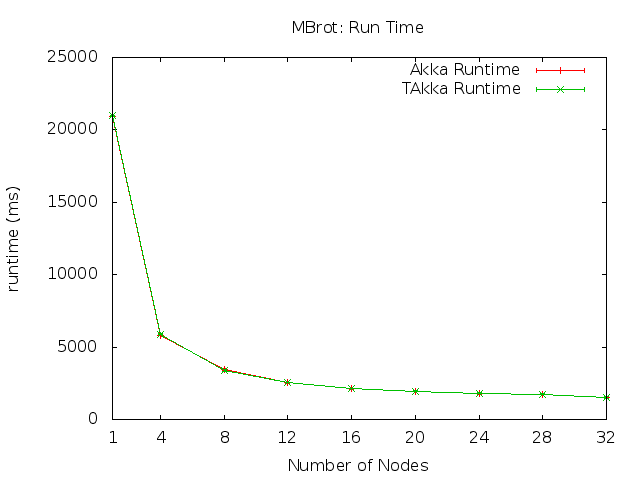
\includegraphics[scale=0.33]{MBrot_time.png}
        }
        \subfigure[]{
           \label{fig:second}
           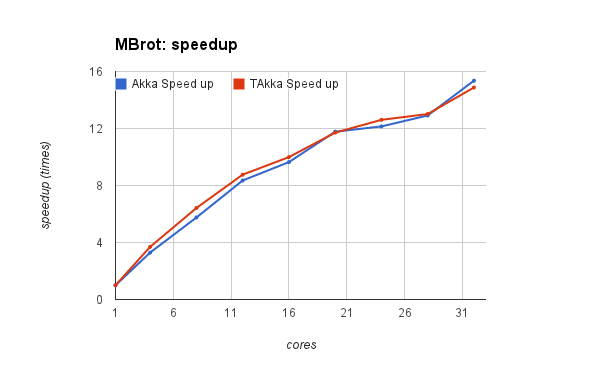
\includegraphics[scale=0.33]{MBrot_speedup.png}
        }\\
        \subfigure[]{
            \label{fig:third}
            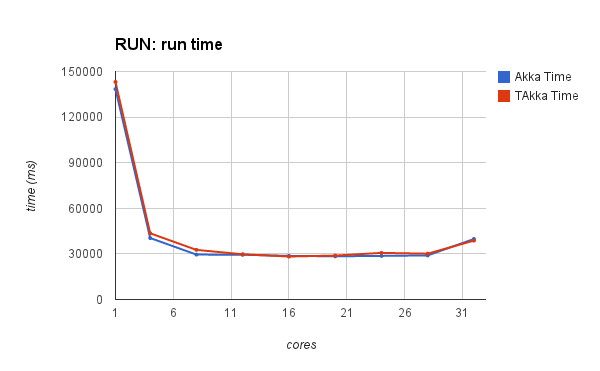
\includegraphics[scale=0.33]{RUN_time.png}
        }
        \subfigure[]{
            \label{fig:fourth}
            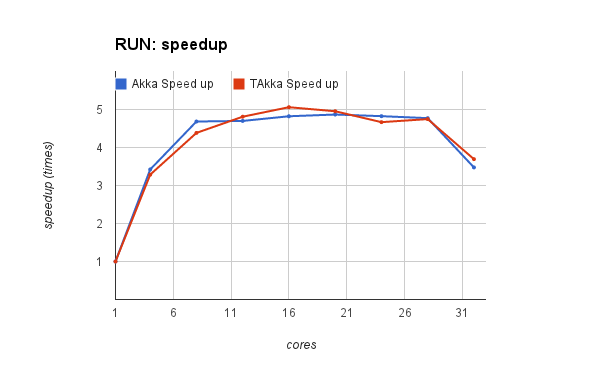
\includegraphics[scale=0.33]{RUN_speedup.png}
        }\\
        \subfigure[]{%
            \label{fig:fifth}
            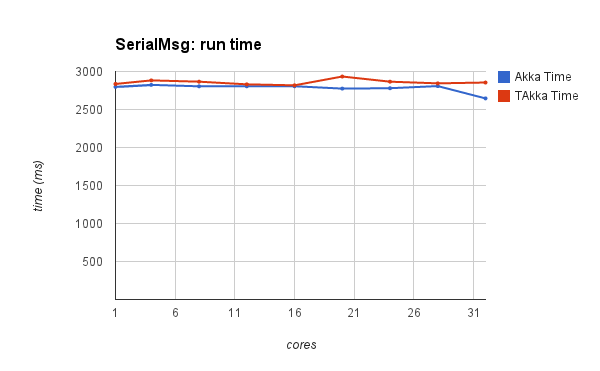
\includegraphics[scale=0.33]{SerialMsg_time.png}
        }
        \subfigure[]{%
            \label{fig:sixth}
            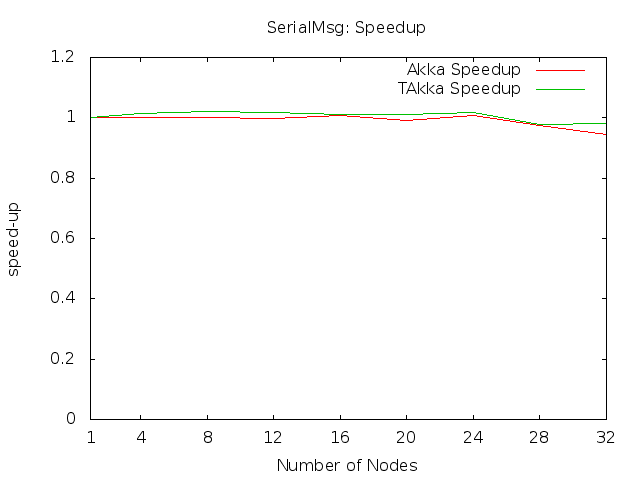
\includegraphics[scale=0.33]{SerialMsg_speedup.png}
        }\\
    \end{center}
    \caption{Efficiency and Scalability Benchmark}
   \label{scalability}
\end{figure}

% \title{Assessing the Reliability \\of\\ Applications with Supervision Tree}
\author{ Jiansen HE }

% \date{\today}
\date{}
\documentclass[12pt, authoryear]{article}

\usepackage{comment}
\usepackage{natbib} 
%% \usepackage[style=alphabetic]{biblatex}
%% \usepackage[authoryear]{natbib}
%% \PassOptionsToPackage{authoryear}{natbib}
%% \usepackage{caption}
\usepackage{graphicx}
\usepackage{subfigure}
\usepackage{subcaption}
\usepackage{url}

\usepackage{paralist}
\usepackage[pdfpagelabels]{hyperref}
\usepackage[all]{hypcap}
\usepackage{verbatim}
\usepackage{array}
\usepackage{float}
\usepackage{multirow}
% \usepackage{rotating}
\usepackage{multicol}
\usepackage{longtable}


\begin{document}
\maketitle

\section{Introduction}\label{introduction}

Libraries such as Erlang OTP \citep{OTP}, Akka\citep{akka_doc}, and TAkka are 
built with the belief that the reliability of a software application can be 
improved by using supervision 
tree, in which failed components will be restarted by their supervisor.  Erlang 
OTP and Akka have been used in a number of applications that have achieved a
high reliability.  Could the reliability of a newly developed 
application be assessed in an effective manner? To what extend the usage of 
supervision tree contributes to the overall reliability?  

To answer above questions, this proposal suggests a research roadmap as follows.
Section \ref{methodology} summarizes general methodologies used in the area 
of reliability studies.  Focusing on the statistic approach to measure the 
reliability of software applications which are expected to have low failure 
rates, we propose to improve \citep{Littlewood93}'s single-run experiment, 
summarized in Section \ref{littlewood}, by using the iterative experiment 
(Section \ref{iterative}) when conditions apply.  The iterative approach can 
reduce the experiment time and can be stopped when the desired belief about the 
reliability had been rejected.  Aside from the methodology for directly 
assessing the reliability of a general application, this proposal also looks 
into approaches that indirectly assessing the reliability of application built 
using the supervision tree principle.   Section \ref{supervision} summarizes 
\citeauthor{JanHenry}'s approach for analysing the statical structure of Erlang 
supervision trees, and Jiansen's extensible work on dynamically monitoring 
TAkka supervision trees.  Finally, the essence of a node in a supervision tree 
is abstracted as a Deterministic Finite Automaton (DFA) in Section \ref{model}. 
The abstraction is used to model and compare designs of supervision tree in 
Erlang and (T)Akka, among alternatives that have not been adopted.  A 
straightforward definition for the reliabilities of a node in a supervision 
tree is derived from the model.  It remains to be seen whether i) the overall 
reliability of a supervising tree can be derived from the reliability of its 
nodes and the structure of that supervision tree, and ii) there exists an 
algorithm to aid the design of supervision tree with a high reliability.




\section{Methodologies for Assessing Software Reliability}\label{methodology}


The reliability in this proposal is defined as the probability that a system can
function properly for a specified period.  Formally, the reliability function, 
$R(t)$, denotes the probability that a system can function properly for time 
$t$.  In the study of software reliability, the period may be specified in term 
of {\it time units} (e.g. second) or {\it natural units} (e.g. number of 
operations) \citep{MusaBook}.  Reliability is usually reported in terms of  
failure rate ($\lambda$), Mean Time Between Failures (MTBF, $1/\lambda$), and 
other variants.  

The reliability function, its failure density function $f(t)$, and MTBF has 
following relationships: \citep{MusaBook}

$R(t) = \int_{0}^{\infty}f(x) dx$

$MTBF = \int_{0}^{\infty} tf(t)dt$

$MTBF = \int_{0}^{\infty} R(t)dt$


In literature, the precise definition of failures varies in the study of 
different systems.  Failure in this proposal is a general term to describe the 
situation where a system or a sub-system does not work as specified.

Once the meaning of failure is defined for a specific application, measuring 
the reliability during a period is straightforward.  The challenge 
is how to use the previous data, collected from experimental or operational 
environment, to give confidence about the reliability in the future under the
operational environment.

For software which involves iterative debugging process, software reliability 
growth models are usually employed to capture the relationship between the bug 
removing process and the reliability improvement.  \citep{Abdel-GhalyCL86} 
examines 10 models in this area, and a framework to evaluate the effectiveness 
of different models.

For software that has reached certain level of reliability and hence 
the debugging process has minor effects, \citep{Littlewood93} gives a 
Bayesian approach to validating its reliability.  Because this approach 
targets at systems that have high reliabilities, we will discuss this approach 
in sufficient detail in the next section.




\section{Statistic Approaches for Measuring Reliability}\label{statistic}

\subsection{Littlewood's approach to predict software 
reliability.}\label{littlewood}

The analysis in \citep{Littlewood93} answers the following question: given 
that $x$ failures are observed during the period of testing $t_0$,  what can we 
conclude about the reliability in the next $t$ time.
  
The two assumptions in Littlewood's approach are:

\begin{enumerate}[{Assumption} I)]
  \item the occurrence of failures is a poisson process, that is, time 
between failures are independent.
  \item the prior belief about the distribution of failure rate, $p(\lambda)$, 
follows the gamma distribution, Gam($\alpha, \beta$), where $\alpha$ and 
$\beta$ are positive hype-parameter that describes the sharp and the rate of 
the distribution.
\end{enumerate}

Assumption I is an appropriate choice for general studies.

Since the posterior belief is adjusted by the observed data, the prior belief 
will have less effect on the posterior belief if sufficient evidence is 
collected from a long experiment.  The Gamma distribution is chosen because it 
is the $conjugate\ distribution$ for poisson distribution.  It means 
that using the Gamma distribution as prior belief will result to a posterior 
belief which also follows the Gamma distribution.  Particularly, if the prior 
belief is Gam($a, b$), then posterior belief will be Gam($a+x, b+t_0$), where 
$x$ is the number of observed failures and $t_0$ is the experiment time. 
\citeauthor{Littlewood93}   Alternatively, any probability distribution may be 
used to replace the Gamma distribution, if it better describes the property of 
the failure rate of a particular application.  



\citeauthor{Littlewood93} then derives that the reliability function for the 
future $t$ time is

$ R(t | x, t_0) = \left ( \frac{b+t_0}{b+t_0+t} \right ) ^{a+x} $


\citeauthor{Littlewood93} then concludes that ``observing a long period of 
failure-free working does not in itself allow us to conclude that a system in 
ultra-reliable'' from the analysis of two extreme cases. 
The first case is, choosing an improper prior so that the posterior completely 
depends on the data.  The posterior itself is an proper distribution; however, 
after observing a period of failure-free operations, one has 50\% possibility 
to be failure-free for the same amount of time in the future.  The second 
example is, to claim a system has $10^6$ hours (114 years) MTBF by showing 
$10^3$ hours (41.7 days) of failure-free working, one must hold the prior 
belief that the system is a $10^6$ system.


\subsection {Reduce experiment time of the Littlewood and Strigini 
 test?}\label{iterative}

In \citeauthor{Littlewood93}'s study, prediction of the reliability is made 
according to the result of an earlier experiment under the same 
operational environment.  In such an experiment, even a long-time failure free 
observation cannot conclude a high reliability for the future. This section 
attempts to solve three problems: i) based on the same assumptions about the 
failure rate, can we improve the experiment so that the expected reliability 
can be verified or rejected earlier? ii) can we validate 
the same basic assumptions used in \citeauthor{Littlewood93}'s and the improved 
approach?  iii) is it possible to claim a genuine prior belief about the 
distribution of the failure rate?


\subsubsection{Iterative experiments}

Assuming that the occurrence of failures is a poission process and the failure 
rate follows the Gamma distribution, representing the Gamma distribution using 
hyper-parameters, it is clear that the posterior belief about the failure rate, 
$Gam(a+x, b+t)$, depends on the prior belief $Gam(a,b)$, the 
$total$ number of observed failures $x$, and the $total$ 
experiment time $t$.  Therefore, for an application that consists of a number 
of replica subsystems, we can replace \citeauthor{Littlewood93}'s experiment 
with an equivalent iterative experiment described below.

An iterative experiment consists of several rounds of sub-experiments, each of 
which may consists of several parallel experiments.  In an iterative 
experiment, the posterior belief of one round is used as the 
prior belief of the next round.  Instead of asking whether a system will be 
reliable in the next $10^6$ hours based on the failure rate of the first $10^3$ 
hours \citep{Littlewood93}, the experiment conductor concerns whether the 
system will be reliable in 
the next round, based on the failure rate of previous results.  In 
each iteration, a number of instances may be tested in parallel to collect the 
results of more instance hours within less time.  An iterative experiment may 
be stopped as soon as the belief about the failure rate is disproved, or the 
base assumption about poisson process and Gamma distribution are rejected.

Take the above proposal into practise, assuming we are asked to test whether 
a distributed web service designed for an organisation will be as reliable as 
its developers claimed for the next a few years.  We may run a test on one or 
two local machines for 1 day.  If the result meets the requirement, then we may 
test the application on some servers of the organisation for half a week.  
Then, we may rent 1000 similar servers from one or more cloud service providers 
in the third round which lasts a week.  By doing this, we can collect the 
number of failures occurred in an experiment of 168,000 instance hours within 
a week ($168,000 = 7 \times 24 \times 100$) .  Fortunately, the data can be 
treated as equivalent to a result 
collected from a single-run experiment on one machine for 19 years ($19 = 
168,000 \div 24 \div 365$) , if our assumptions are valid for tested system.  
Renting a thousand server instances might be expensive, but the risk of wasting 
resource on testing application that doesn't meet the desired reliability has 
been reduced in previous rounds of tests.


\subsubsection{Verify Assumptions}

Both \citeauthor{Littlewood93}'s original approach and our alternative are based 
on the assumption that the occurrence of failures is a poisson process and the 
failure rate follows a Gamma distribution represented by two 
hyper-parameters.  Those two assumings are good choice in a study for general 
purposes.  For a test of a real application, to what extend can we rely on the 
assumption of poisson process and the prior belief with guessed 
hyper-parameters?  To verify those assumptions, suitable goodness-of-fit tests 
can be used.  Following are example approaches.


To verify the assumption on poission process, we can alternatively check 
whether the number of failures in consecutive fixed periods follows the 
poission distribution, whose mean and variance are the same.  To verify the 
assumption on gamma distribution, \citep{GammaFIT} gives improved methodologies 
for the purpose of reliability test.


\subsubsection{Obtain a genuine prior belief}

Following is my guesswork. Appropriate statistic analysis is required.

If $x$ failures are observed in the previous experiment of $t$ time and the 
base assumption cannot be rejected by the data in previous tests, the 
{\bf best} prior belief for the next iteration is assuming the distribution of 
failure rate $\lambda$ follows Gam($x$, $t$).

This is a significant difference between the iterative experiment and 
\citeauthor{Littlewood93}'s single run experiment.  In 
\citeauthor{Littlewood93}'s approach, claiming a Gam($x$, $t$) {\it posterior} 
is the same as claiming a improper $prior$ Gam($a$, $b$), where $a,\ b\ 
\rightarrow 0$.  In an iterative experiment, the first round can be used to 
``generate'' a reliable prior for the second round.  However, at least 1 failure 
need to be observed in the first round because $a$ and $b$ in Gamma distribution 
are positive numbers.  In a ultra-reliable system, waiting for the first 
occurrence of failure may take a long time.


\subsubsection{Testing in adversely environment.}

Another attempt to give a reliability prediction in short period is testing 
the system in adversely environment.  This idea, known as accelerated testing 
(AT), has been explored in hardware reliability test for years 
\citep{Escobar06areview}, and has been applied to test the $FASTAR^{SM}$ 
platform, a set of systems used to automatically  restore the AT\&T 
network\citep{CukicSoft}.

An accelerated test consists of two general steps.  The first step is to 
identify accelerating factors (e.g. temperature, workload, temperature etc.) and 
run the experiment.  The second step is to use suitable regression model to 
predict the reliability in normal condition.  

The significance of an accelerated testing depends on the choice of the 
regression model.  For a hardware, the relationship between its life-time 
and environment factors (e.g. temperature) has been well studied.  In the 
$FASTAR^{SM}$ test, to capture and verify the regression model, 32 runs are 
carried out under different pressure environment.  Each run lasts for about 30 
hours and a few failures are observed during the test.  

Bring in the same idea into the test of TAkka applications, for example, with 
the help of the Chaos Monkey library, can we effectively test the reliability 
within a reasonable short period?  Unfortunately not.  

Let's run two experiments in parallel.  In one experiment, ChaosMonkey is not 
used and its failure rate, $\lambda_n$, is assumed to be the same as in the 
normal operational environment. In the other experiment, ChaosMonkey is 
employed to increase the exception rate so that the failure rate, $\lambda_c$, 
will be higher than $\lambda_n$.  Failure rates in the two experiments are 
linked by the following equation:
$\lambda_n \times t_n = \lambda_c \times t_c$, where $t_n$ and $t_c$ are expect 
periods of seeing $x$ failures in the normal environment and in the ChaosMonkey 
test.

The above equation shows that the expected time for the $nth$ occurrence of 
failures decreases when its failure rate increased.  Therefore, assumptions 
on the poission process and the Gamma distribution can be verified in shorter 
time.  From a serials of ChaosMonkey test with different failure rates, we may 
fortunately find that the occurrence of failures in the tested application is 
always a poission process.  As a result, to measure its reliability in normal 
operational environment, only a small number of errors need to be observed 
under the test in normal environment.  However, it may take a long time to 
observe the first occurrence of failures in a system whose MTBF is $10^6$ 
hours.




\section{Reliability Studies on Supervision Tree}\label{supervision}

\subsection{Static Analysis on Tree Structure}\label{Static}

Based on the Core Erlang Language defined by \citep{CoreErlang}, 
\citep{JanHenry} defines an abstract semantic to extract structures of Erlang 
programs.  Since supervision tree is constructed in Erlang by calling callback 
functions in the {\it supervision} module, \citeauthor{JanHenry}'s work can 
be used to abstract the structure of supervision trees form the source code of 
Erlang applications.

Noted in the later part of \citeauthor{JanHenry}'s thesis, there are two 
limitations of his approach.  Firstly, the abstraction only captures the static 
structure of the supervision tree, which may differ from its run-time 
structure.  Secondly this approach requires specialised knowledge about the 
Erlang language and only applies to ``applications that have been 
designed according to the suggestion of the OTP documentation and using the OTP 
library behavious.'' \citep{JanHenry}.



\subsection{Dynamic Monitoring}\label{Dynamic}

The supervision view library in the TAkka paper.




\section{Modelling Supervision Tree}\label{model}


To study properties of supervision tree, a simple formal model is required to 
describe the essence of supervision tree.  Section \ref{DFA}
models Worker and Supervisor and Deterministic Finite Automata (DFA).  With 
this model, implementation alternatives of Supervision Tree are compared.  More 
importantly, the model helps us to give a simple general definition for the 
reliability of nodes in a supervision tree.  This section ends with a proposal 
for investigating the reliability of a supervision tree, based on the 
reliabilities of its nodes and the relationships between nodes.


\begin{comment}
The model shall not include 

The model shall contain the minimum 
number of constructs and small-step semantics that describes supervision.  
Operations related to supervision are separated from functions and 
message-passing for general purpose.  The simple model will be used to compared 
core Erlang (where supervision is optional), Akka (where supervision is 
obligatory), and TAkka (where messages are typed).  Since Akka and TAkka don't 
have a formal model, giving a model that can be used to describe/check their 
properties is a non-trivial contribution.


In addition, a stack of failure models will be defined.  We will examine 
failures that are typically handled at hardware level, OS level, VM level, and 
the application level.  Presumably, supervision injects a layer between the 
application and the VM, and automates the recovery of some failures previously 
handled by programmers at the application level (e.g. exception).
\end{comment}

\subsection{Worker and Supervisor as Deterministic Finite Automata (DFA)} 
\label{DFA}

Figure \ref{fig:DFA} gives state graphs of DFAs that describe 
worker and supervisor in a supervision tree.  Nodes in the graphs represent 
states of that DFA and arrows are transitions from one state to another.  A 
transition is triggered either by the node itself or due to changes of the 
environment it resides.

At any time, a worker may be in one of its four states: {\bf Start}, {\bf 
Free}, {\bf Blocked}, or {\bf Dead}.  After automatically being initialised to 
the {\bf Free} state, the Work can accept messages from its outside 
environment and enters to the {\bf Blocked} state where no messages will be 
processed.  If no error occurred when processing the message, the worker emits 
a result and go back to the {\bf Free} state.  An error may occur during the 
middle of message processing (e.g. software bugs) or when the environment 
changes (e.g. hardware failures), in which cases the worker reports its failure 
to its supervisor and go to the {\bf Dead} state.  A dead worker can be resumed 
or restarted by its supervisor so that it can process new messages.  {\bf Free} 
and {\bf Dead} are marked as accept states from which no further actions may 
occur.  On the contrary, a {\bf Blocked} worker will eventually emit a reply 
message or raise an exception; and all workers will be successfully initialised.

The DFA of a supervisor whose only duty is supervising its children is given in
Figure \ref{fig:2}.  A supervisor in its {\bf Free} state reacts to failure 
messages from its children.  Meanwhile, a supervisor may fail at any time 
and reports its failure to its supervisor.

\begin{figure}[p]
     \centering 
        \subfigure[Worker]{
            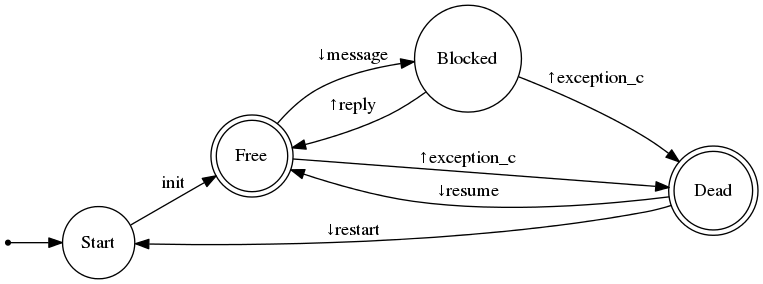
\includegraphics[scale=0.5]{child.png}
%            \caption{A gull}
            \label{fig:1}
        }\\
        \subfigure[Supervisor]{
           \label{fig:2}
           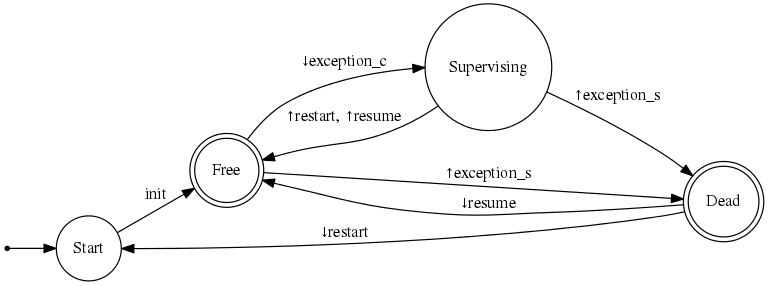
\includegraphics[scale=0.5]{supervisor.png}
        }\\
  \caption{Worker and Supervisor as Deterministic Finite Automata}
  \label{fig:DFA}        
\end{figure}

\subsection{Implementation Considerations}

The two DFAs given in Figure \ref{fig:DFA} are abstracted for theoretical 
study.  In an implementation of the supervision tree model, following issues 
might be considered.

\paragraph{Distributed Deployment}
Supervision Tree represents the logic relationship between nodes.  In 
practice, nodes of a supervision tree may be deployed in distributed machines.  
A child node may be restarted at or shipped to another physical or virtual 
machine but stays in the same place in the logic supervision tree.


\paragraph{Heart-Beat Message}  At run-time, failures may occur at any time for 
different reasons.  In some circumstances, failure messages of a child may not 
be delivered to its supervisor, or even worse, not sent by the failed child at 
all.  To built a system tolerant to the above failures, supervisors need to be 
aware of the liveness of their children.  One approach to achieve this is 
asking the child periodically sending heart-beat message to its supervisor.  
If no heart-beat message is received from a child for some consecutive 
periods, that child is considered dead by the supervisor and an appropriate 
recovery process is activated.  In the model, a 
logical exception is sent from a child to its supervisor when no heart-beat 
message is delivered within a time-out, and a restart or resume message is sent 
to a suitable machine where the node will reside.


\paragraph{Message Queuing}
In the simplified model given in Figure \ref{fig:1}, a worker can processed one 
message a time when it is {\bf Free}.  The model does not exclude the case 
where messages are queuing either in memory or a distributed database.  
Similarly, when a worker is resumed from the failure of processing a message, 
the message it was processing may be retrieved from a cache or be discarded.




\subsection{Unifying Supervisor and Worker}

Notice that the model for supervisor and worker are similar if exceptions from 
the child is viewed as request messages to a supervisor and restart/resume 
is viewed as reply messages to a child.  Can we defined a $combined$ node which 
can be both a worker for a task and a supervisor for some children? Of course 
we can, as what have been implemented in Akka\citep{akka_doc} and inherited by 
TAkka. The rest of this sub-section will compare three strategies of unifying 
supervisor and worker.

\paragraph{Supervisor as a Worker}  In the design of Akka, messages to 
actors are not typed.  An Akka actor therefore can be both a supervisor and a 
worker.  To model an Akka actor, only Figure \ref{fig:1} is required.

\paragraph{Combining Supervisor and Worker}  The TAkka library inherits the 
implementation of Akka, but separates messages for supervision purpose from 
messages for general purposes so that an actor can be parameterized by the 
type of message it expects.  A more precise model for a TAkka actor is given in 
Figure \ref{fig:3}.  Both Akka actor and TAkka actor can only be a supervisor 
or a worker at a time.  As a result, the supervision task may be blocked until 
the end of another computational task.


\paragraph{Supervisor in Parallel with Worker}  One way to get around the 
limitation of Akka and TAkka's design is place the supervision process and the 
worker process in parallel, as shown in Figure \ref{fig:4}.  From the 
perspective of model analysis, the above parallel model is equivalent to the 
one which separates the supervisor process and the worker process into two 
nodes, and treat them as siblings or a supervisor and a child.



\begin{figure}
%  \ContinuedFloat 
  \centering         
        \subfigure[Supervisor AND Worker]{
            \label{fig:3}
            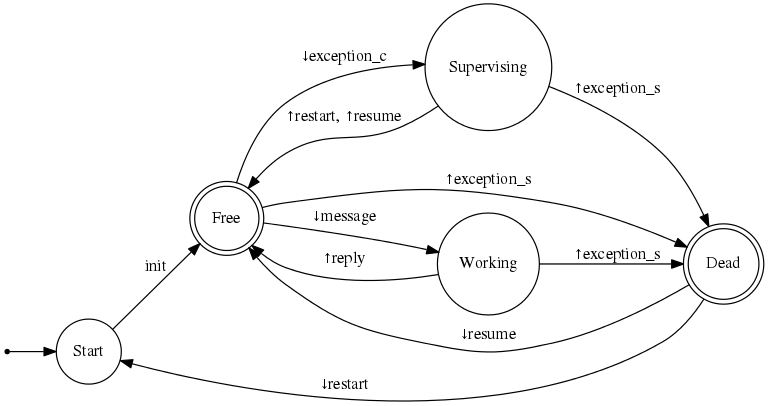
\includegraphics[scale=0.5]{supervisorANDchild.png}
        }\\
        \subfigure[Supervisor PAR Worker]{
            \label{fig:4}
            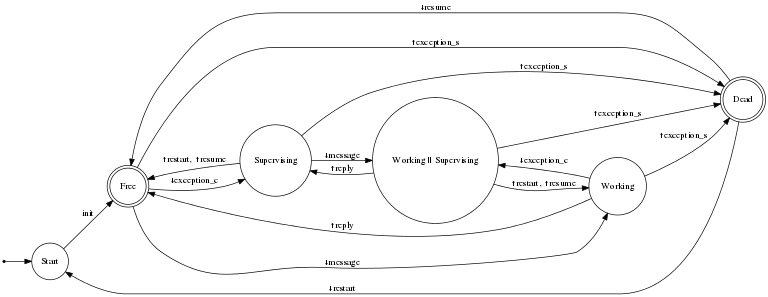
\includegraphics[scale=0.5]{supervisorPARchild.png}
        }\\
    \caption{A Node that Unifies Supervisor and Worker}
   \label{fig:unify}
\end{figure}


To summarize, a node that naively combining the role of supervisor and worker 
(Figure \ref{fig:1} and \ref{fig:3}) has less availability than a node that 
place the supervision process and the worker process in parallel processes 
(Figure \ref{fig:4}).  Interestingly, during the process of designing TAkka, we 
realized that the type of supervision messages should be separated 
from the type of other messages.  However, partly because we would like to 
reuse the Akka implementation and partly because we did not have the above 
model at that time, the process of handling supervision messages is not 
separated from the process of handling other messages.


\subsection{Reliability of a Node}

The reliability of a node, either a worker or a supervisor, is defined as:

The the probability that a node is in the {\bf Free} state.


\subsection{Reliability of a Supervision Tree}

A supervision tree in this proposal consists of workers and supervisors defined 
in Figure \ref{fig:1} and Figure \ref{fig:2} respectively.  A node that 
combines a supervisor and a worker is separated into two nodes, together with a 
constraint that one node will fail when the other fails.

The reliability of a supervision tree may be derived from following factors:

\begin{itemize}
  \item The reliabilities of all workers.  Although testing the reliability of 
a system with low failure rate is difficult or even impractical, the 
reliability of an individual component may be measured within a reasonable 
short time. 
  \item The reliability of a supervisor.  The reliability of a supervisor 
process may be tested as part of the library development process.
  \item The relationship between nodes.  Nodes in a supervision tree may 
collaborate to perform a task or to achieve a higher reliability. The 
reliability of a supervising shall capture complex relationships 
between nodes.
\end{itemize}

The experiment proposed in section \ref{iterative} may to used to measure the 
reliabilities of individual nodes in a supervision tree.  To obtain the 
reliability of a supervision tree, when direct measurement becomes impractical, 
knowledge about constraints between nodes are required.  

I propose to investigate following problems in the next stage:

\begin{itemize}
  \item What are possible constraints between nodes?  For each constraint, what 
is the algebraic relationship between the reliability of a sub-tree and 
reliabilities of individual nodes?
  \item Based on the above result, how to calculate the overall reliabilities 
of a supervision tree?  When is the reliability is improved by using 
supervising tree, and when not?
  \item Given the reliabilities of individual workers and constraints between 
them, is there an algorithm to give a supervision tree that improves the 
reliability?  If not, can we determine if the desired reliability is not 
achievable? 
\end{itemize}


\bibliographystyle{abbrvnat}
\bibliography{reliability}

\end{document}




\acks


The authors gratefully acknowledge the substantial help they have received from 
many colleagues who have shared their related results and ideas with us over 
the long period during which this paper was in preparation.  
Benedict Kavanagh and Danel Ahman for continuous comments and discussions.
The RELEASE team for giving us access to the source code of the BenchErl 
benchmark examples.  Thomas Arts from Quviq.com and Francesco Cesarini from 
Erlang Solutions for providing the Erlang source code of two examples used in their 
commercial training courses.

\vspace{-10pt}


% ---- Bibliography ----
\bibliographystyle{abbrvnat}
\bibliography{takka}

\end{document}
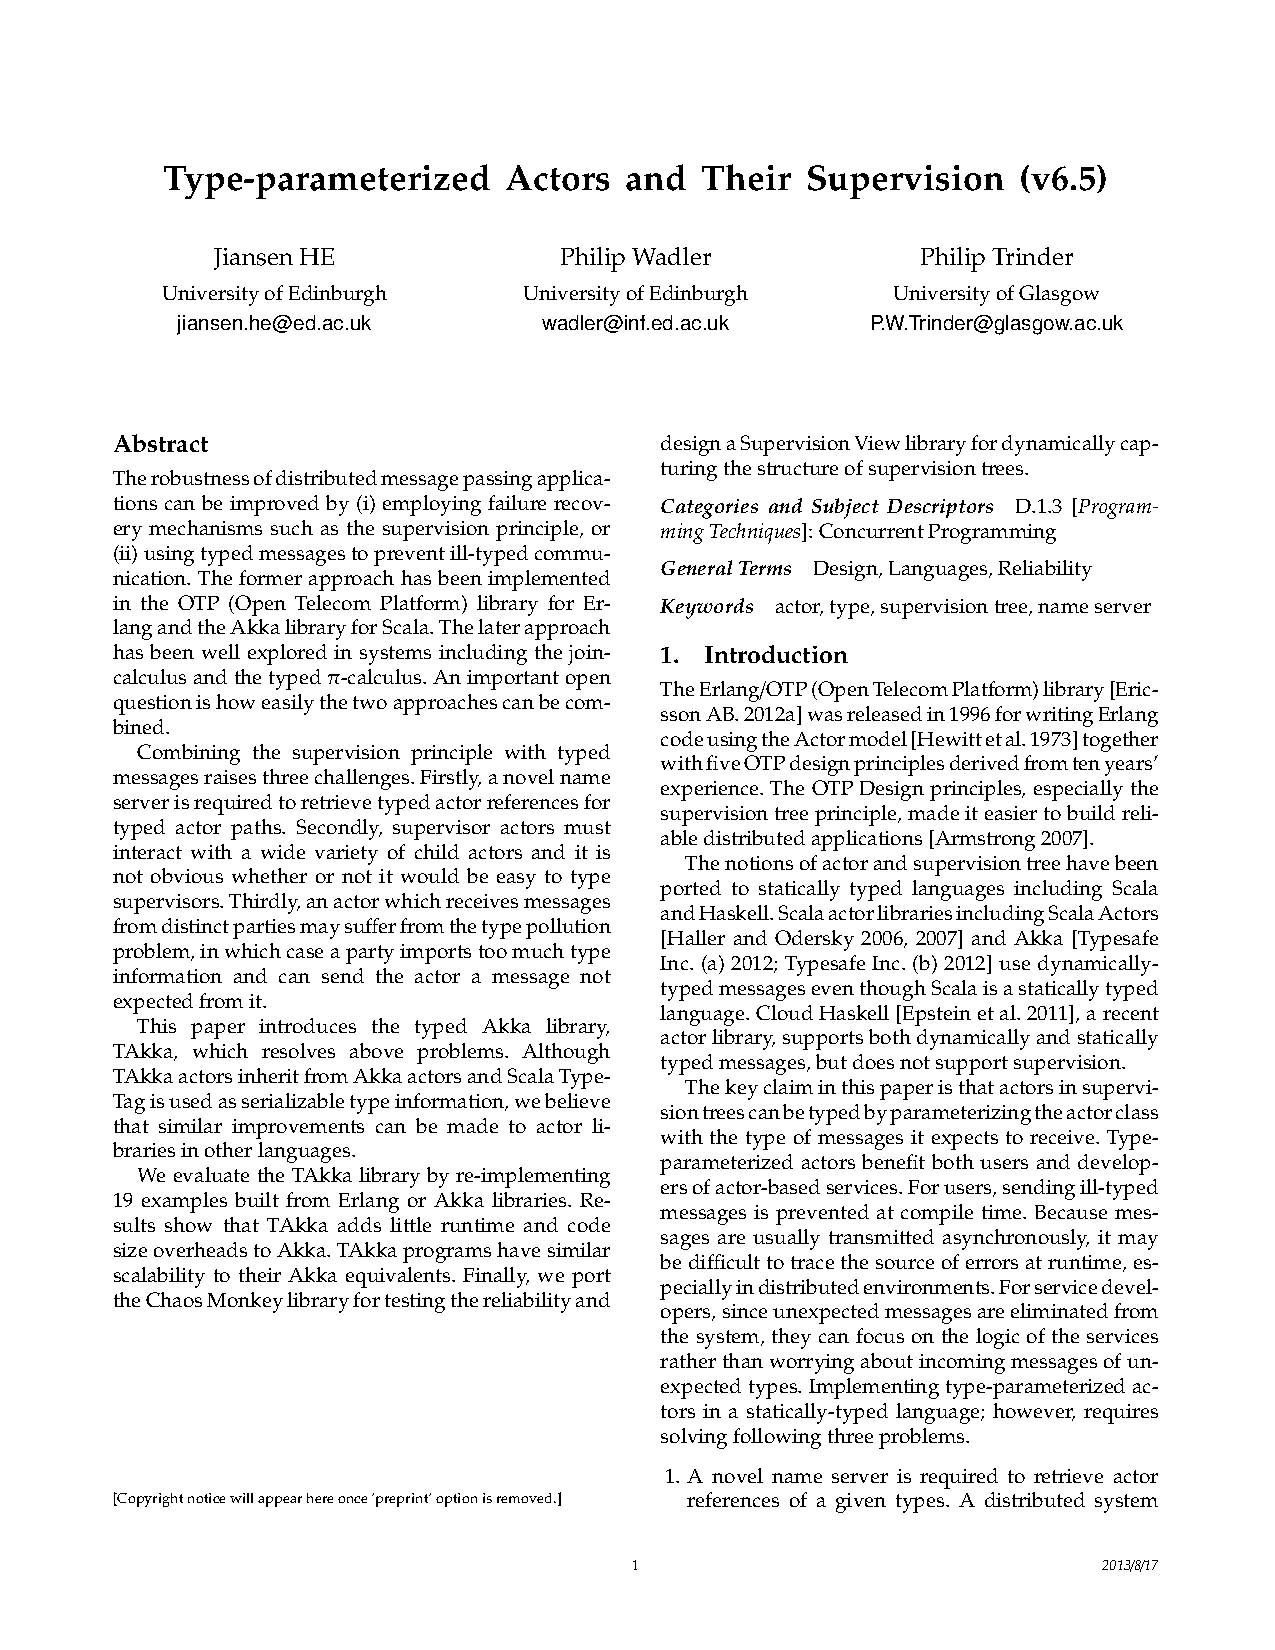
\includepdf[pages={1-20}]{takka.pdf}
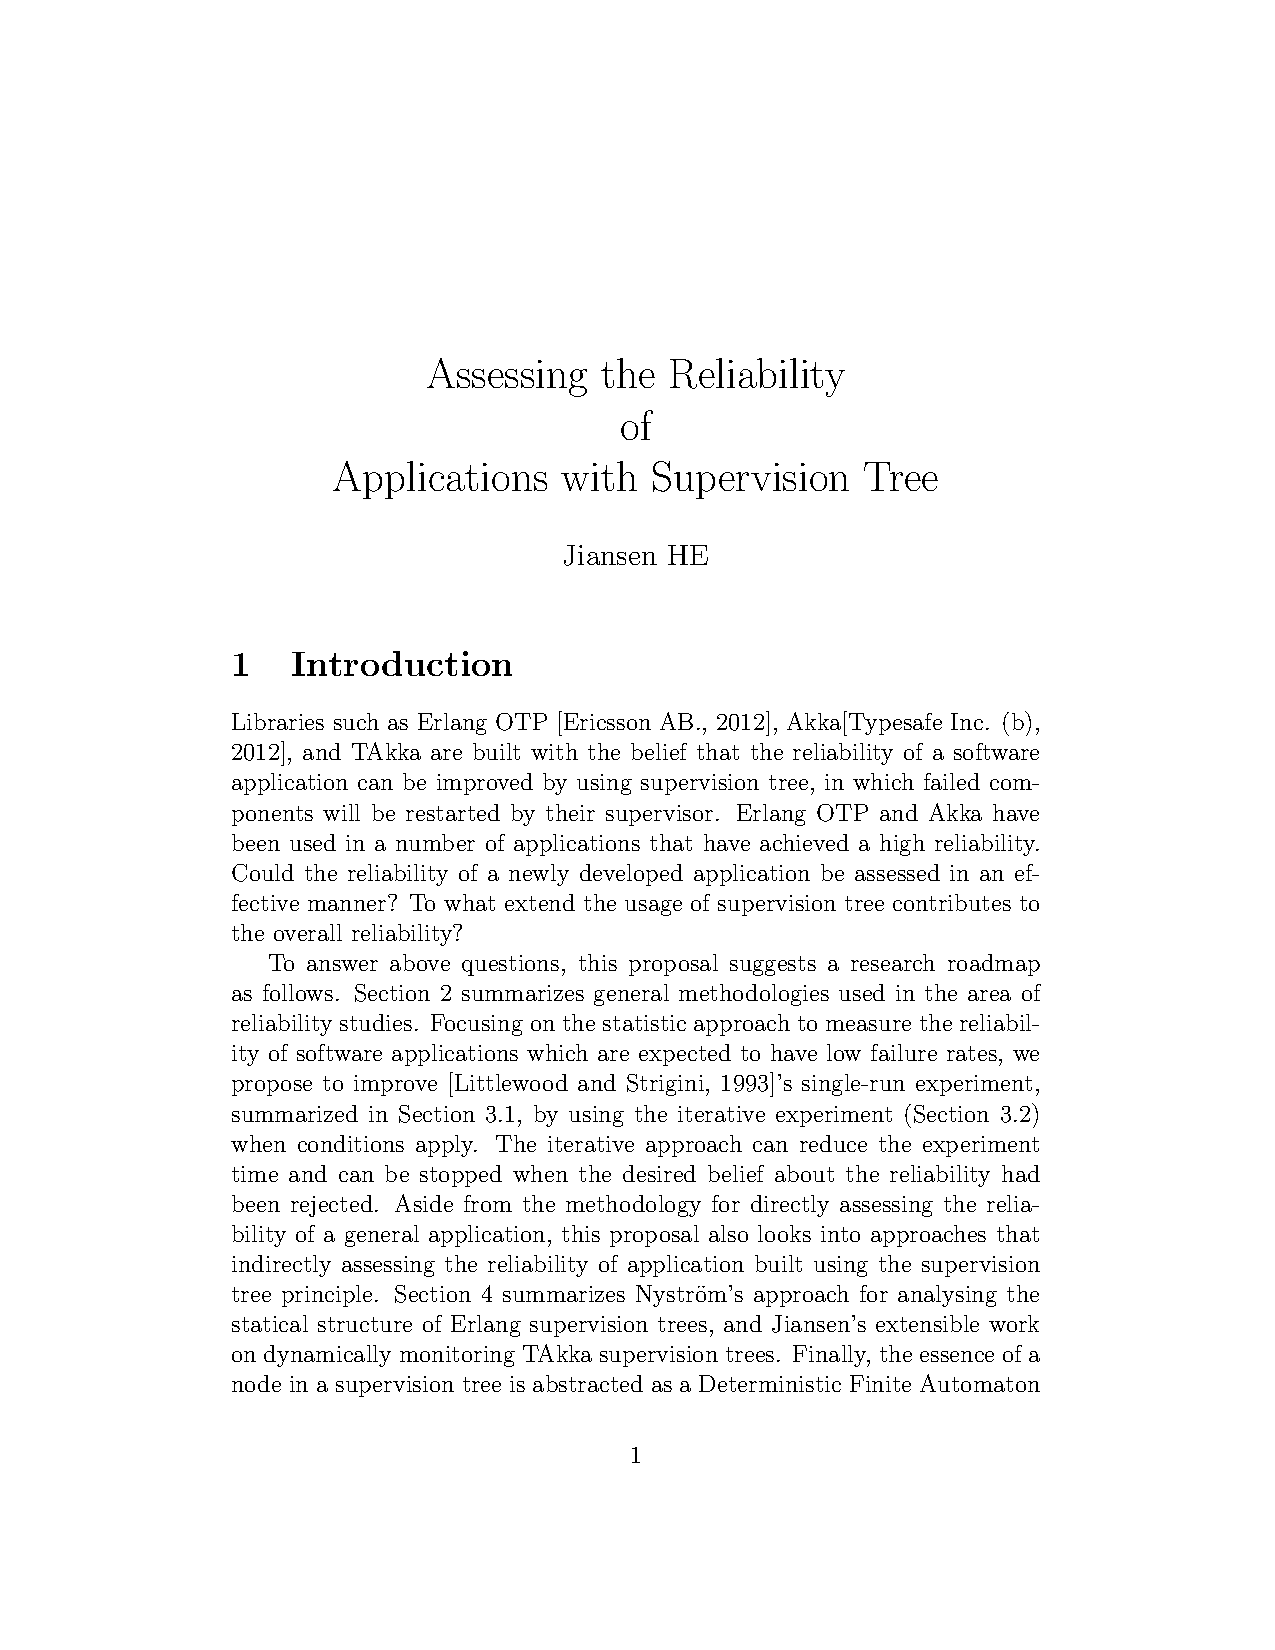
\includepdf[pages={1-14}]{reliability.pdf}

\end{document}
